\documentclass[../main.tex]{subfiles}
\graphicspath{{\subfix{../../images/}}}
\begin{document}

\chapter{Theoretical Background}\label{chap:bg_theory}

\begin{quote}
  \emph{Even a simple movement is a global body event.}
  --- Bizzi \& Ajemian, \emph{2020}
\end{quote}  


\begin{quote}
  The processes by which biological control solutions spanning large and continuous state spaces are constructed remain relatively unexplored. Future investigations may need to embed rich dynamical interactions between object dynamics and task goals in novel and complex movements
  \cite{McNamee2019}.
\end{quote}


Framing 
    

\section{Background Theory}\label{background-theory}

From the physiology, we see that the motor system is highly distributed
and constructs action based on a variety of state dependence. The
theoretical question becomes \emph{when does it make computational sense
to construct action by composing control policies rather than selecting
or tuning a single policy?} When is policy arbitration computationally
advantageous?

\textbf{The motor learning field does not yet possess an adequate
computational model for practice-induced increases in motor acuity.}
(Krakauer Motor Learning 2019)

\subsection{Existing Models of Motor Control and
Adaptation}\label{existing-models-of-motor-control-and-adaptation}

\subsubsection{Optimal Feedback Control}\label{optimal-feedback-control}

Stephen Scott review -- https://www.nature.com/articles/nrn1427 look at
the bullet points there, relate to our experiment

OFC is the best we got for motor coordination, but there's no adaptation
or learning

The control setup writes a cost, environment has some dynamics.

What is changing in this scenario? What is being learned? What
information is used to do this learning?

Which model variables correspond to muscles? Movements? What does the
resultant feedback controller compute? How does this relate to
cognition?

This model is lacking in \ldots{}

A key paper is \texttt{Valero-Cuevas\ 2009} which recording EMG from the
seven muscles driving the finger in a force-feedback task. The authors
found support for the ``minimum intervention principle''
{[}@Valero-Cuevas2009{]}.

\subsubsection{nonlinear iLQG models}\label{nonlinear-ilqg-models}

these are more predictive if we're actually using reaches experimentally

nagengast, braun, etc 2009
https://journals.plos.org/ploscompbiol/article?id=10.1371/journal.pcbi.1000419

\subsubsection{Noise in OFC}\label{noise-in-ofc}

\begin{itemize}
\tightlist
\item
  Nagengast 2010
  https://journals.plos.org/ploscompbiol/article?id=10.1371/journal.pcbi.1000857
  -- subjects are risk averse in the face of noise.
\end{itemize}

\subsubsection{Intuitive Example of the OFC
framework}\label{intuitive-example-of-the-ofc-framework}

Here we see a feedback controller with three muscles such that we can
plot the muscle activation trajectory.

This is the feedback controller K, we can understand it's action by
plotting

PLOT OF SIMPLE EXAMPLE

PLOT OF APT DATA

\subsubsection{Error-based Adaptation}\label{error-based-adaptation}

Error-based adaptation and state-space models have a great amount of
precedent in the sensorimotor learning literature. We will summarize
these models briefly and discuss our willingness to depart from them.

This is pretty much the best model we have that describe learning from
error

Current models of motor learning

x' = Ax + Bu

This model describes\ldots{}

The downsides of this model are that it describes a small aspect of our
data.

\subsection{Adaptive Linear Quadratic
Control}\label{adaptive-linear-quadratic-control}

Have to be careful about what is termed corrective, adaptive, and
learned.

\begin{quote}
Mathematically, we can formalize an adaptive control problem as a
mapping x t+1 = F(x t , u t , a) with unknown system parameters a that
have to be estimated simultaneously with the control process (Sastry and
Bodson, 1989; Åström and Wittenmark, 1995). (Braun 2009\ldots{} Wolpert)
\end{quote}

\begin{quote}
In the following we will refer to changes in the control policy that
occur within individual movements as ``adaptation'' to distinguish them
from ``learning'' processes that improve these adaptive responses across
trials. (Braun 2009\ldots{} Wolpert)
\end{quote}

\begin{quote}
Online correction is, for example, required in the case of an
unpredicted target jump. Under this condition the same controller can be
used, i.e., the mapping from sensory input to motor output is unaltered.
However, unexpectedly changing the hand--cursor relation (e.g., by a
visuomotor rotation) requires the computation of adaptive control
policies.
\end{quote}

\begin{quote}
Strictly speaking, an adaptive control problem is a nonlinear control
problem with a hyper-state containing state variables and (unknown)
parameters. This means in principle no extra theory of adaptive control
is required. In practice, however, there is a well established theory of
adaptive control (Sastry and Bodson, 1989; Åström and Wittenmark, 1995)
that is built on the (somewhat artificial) distinction between state
variables and (unknown) parameters. The two quantities are typically
distinct in their properties. In general, the state, for example the
position and velocity of the hand, changes rapidly and continuously
within a movement. In contrast, other key quantities change discretely,
like the identity of a manipulated object, or on a slower timescale,
like the mass of the limb.
\end{quote}

We're really interested here in the learning problem! And how we can
test and model this within the framework of OFC.

\subsection{Motor Adaptation}\label{motor-adaptation}

Implicit / Explicit Model-based / Model-free Slow / Fast

Krakauer et al.'s categorization of motor learning places prior work
into the following classes: - Adaptation - Sequence Learning - De Novo
Learning - Motor Acuity - Expertise

work in reaching shadmehr, krakauer reviews

\subsubsection{State-space Models of Motor
Adaptation}\label{state-space-models-of-motor-adaptation}

\emph{Modeling Sensorimotor Learning with Linear Dynamical Systems} by
Cheng and Sabes, 2006. The goal is to model trial-by-trial learning by
fitting data to a linear dynamical system model. Here we'll call \(F_t\)
the \textbf{sensorimotor mapping} transforming inputs \(w_t\) to \(y_t\)
outputs per trial:

\[
y_t = F_t(w_t, \gamma_t).
\]

This can be thought of as a mapping from inputs within a single trial
to, for example, endpoint error. Noise is captured by the \(\gamma_t\).
The trajectory in \(F\) space attempts to capture the process of
learning. The learning rule \(L_t\) can be written

\[F_{t+1} = L_t\left(\left\{F_\tau\right\}_{\tau=1}^{t}, u_t, \eta_t, t\right)\]

where \(\left\{F_\tau\right\}_{\tau=1}^{t}\) is the history of the
mapping, \(u_t\) is the history of the total inputs to learning which
could encompass \(y\), \(w\), and exogenous inputs \(r\). Noise in the
learning is captured by \(\eta\).

We can approximate this learning problem using linear equations by
assuming that \(L_t=L \ \forall \ t\) is stationary, \(F_t\) is
parameterized by \(x_t\in\mathbb{R}^y\). Thus,

\[
\begin{aligned}
y_t &= F(x_t, w_t, \gamma_t) \\
x_{t+1} &= L(x_t, u_t, \eta_t).
\end{aligned}
\]

The trial-to-trial input-output mapping \(F\) is now fixed, and is
transformed by trial through its parameters \(x_t\) by \(L\). Note that
both mappings are Markovian and there are two input vectors, one for
within-trial and one between-trial. These can include overlap. We can
now linearize these mappings around an equilibrium point:

\[
\begin{aligned}
x_{t+1} - x_e &= A(x_t-x_e) + B(u_t-u_e) + \eta_t \\
y_t - m_e &= C(x_t-x_e) + D(w_t-w_e) + \gamma_t
\end{aligned}
\]

As shown by Cheng and Sabes, we can bundle the equilibrium terms into a
bias term and drop this term if we mean-subtract our data
(\(x_t, y_t, u_t, w_t\)) when it's time to fit. This gives us a simple
linear dynamical system:

\[
\begin{aligned}
x_{t+1} &= Ax_t + Bu_t + \eta_t \\
y_t &= Cx_t + Dw_t + \gamma_t.
\end{aligned}
\]

The first equation governs the evolution of parameters of the
within-trial input-output mapping, while the second equation governs the
trial output given the current within-trial mapping parameters \(x_t\)
and learning inputs \(w_t\). The parameters \(x_t\) are hidden variables
that are only observed through the output \(y_t\). The noise terms
\(\eta_t\) and \(\gamma_t\) are normally distributed with covariances
\(Q\) and \(R\), respectively. \(A\) governs the passive trajectory of
\(x_t\). If \(A=\mathbb{I}\), \(x_t\) does not decay passively.

There is a general form for this model which separates endogenous input
\(y_t\) from exogenous input \(r_t\)

\[
\begin{aligned}
x_{t+1} &= Ax_t + [G \ H][r_t \ y_t]^T + \eta_t \\
y_t &= Cx_t + Dw_t + \gamma_t
\end{aligned}
\]

where \(H\) governs biases in directions of the outputs. A unbiased
output is isotropic. To add explicit stationary bias we write

\[
\begin{aligned}
x_{t+1} &= Ax_t + Gr_t + Hy_t - Hb_x + \eta_t.
\end{aligned}
\]

\subsubsection{Example Models}\label{example-models}

\paragraph{Feedback Error Learning}\label{feedback-error-learning}

\[x_t+1 = Ax_t + [H\ H][-y_t^*\ y_t]^T\]

The second term is simply the difference between the output \(y_t\) and
the desired output \(y_t^*\).

\paragraph{Prediction Error Learning}\label{prediction-error-learning}

Let \(u_t = y_t - \hat{y}_t\) where \(\hat{y}_t\), the difference
between the output and the predicted output such that

\(\hat{y}_t = Cx_t + Dw_t\). Thus,\(\hat{y}_t\) is a kind of forward
model. Plugging in,

\[x_{t+1} = Ax_t + Bu_t + \eta_t\]

becomes

\[
\begin{aligned}
x_{t+1} &= Ax_t + B(y_t - Cx_t - Dw_t) + \eta_t \\
x_{t+1} &= (A-BC)x_t + By_t - BDw_t + \eta_t
\end{aligned}
\]

\paragraph{Target Prediction Error
Learning}\label{target-prediction-error-learning}

Now let \(u_t = \hat{y}_t - y^*_t\), the difference between predicted
output and target output.

\[
\begin{aligned}
x_{t+1} &= Ax_t + B(Cx_t + Dw_t - y^*_t) + \eta_t \\
x_{t+1} &= (A+BC)x_t + BDw_t - By^*_t + \eta_t
\end{aligned}
\]

\paragraph{Steady State}\label{steady-state}

If we take the output and state vectors in expectation for constant
inputs \(w\) and \(r\), we have

\[
\begin{aligned}
y_\infty &= \lim_{t\to\infty}\mathbb{E}\left[Cx_\infty + Dw\right] \\
x_\infty &= \lim_{t\to\infty}\mathbb{E}\left[Ax_\infty + Bu\right] \\
&= Ax_\infty + Gr + Hy_\infty \\
&= Ax_\infty + Gr + HCx_\infty + HDw \\
-(A + HC - \mathbb{I})x_\infty &= HDw + Gr.
\end{aligned}
\]

Thus, the eigenvalues of \(A + HC\) must be less than or equal to 1 for
\(x_\infty\) to be stable in expectation.

\subsubsection{Critique}\label{critique}

\begin{quote}
It should be emphasized, however, that these models are not intended to
provide a mechanistic explanation of adaptation---they do not explain
why adaptation has the properties it does. They explain neither why
compensation for a perturbation decays, nor why people learn at the rate
they do. However, these models do encapsulate a set of simple
assumptions about how learning might occur on a single-trial timescale,
and allow us to predict behavior in response to sustained or fluctuating
perturbations over many trials. (Krakauer)
\end{quote}

\begin{quote}
{[}Bayesian theories of learning{]} hold that adaptation is essentially
a problem of estimating the properties of the imposed perturbation,
given uncertainty about sensory feedback and the state of the world.
Mathematically, under certain assumptions (that the noise/variability is
Gaussian in both cases), this Bayesian estimation framework becomes
equivalent to a Kalman filter (219)---a common algorithm for optimally
tracking dynamic states under noisy observations--- which is almost
identical to a state-space model. (Krakauer)
\end{quote}

\subsection{Two-rate models}\label{two-rate-models}

\[
\begin{aligned}
X_{t+1} &= X^{s}_{t} + X^f_t \\
X^s_{t+1} &= L_s \cdot e_t + R_s \cdot X^s_{t} \\
X^f_{t+1} &= L_f \cdot e_t + R_f \cdot X^f_{t} \\
\end{aligned}
\]

where we fit \(L_i and R_i\), the learning rate and retention
parameters. (shadmehr 2006)

\begin{quote}
Observations have revealed that there is far more to how participants
compensate for an imposed perturbation than just implicit recalibration
of a pre-existing motor controller. Instead, multiple, qualitatively
different processes occur during adaptation tasks; for example,
processes driven by explicit, cognitive strategies. When it comes to
studying implicit recalibration, these other processes can be a
contaminant. At the same time, however, these additional processes
likely reflect the involvement of similar mechanisms to those
responsible for more general motor skill learning. (Krakauer 2019 Motor
Learning Review)
\end{quote}

\begin{quote}
it is unlikely that the underlying components that contribute to
learning in adaptation paradigms only differ in terms of their learning
and retention rates, as the two-state model suggests. The multiple
components of learning instead correspond to entirely distinct learning
processes that are simultaneously brought to bear on the same problem.
(Krakauer 2019 Motor Learning Review)
\end{quote}

%  The UCM is not a hard-and-fast principle, as nothing as in the motor system. Rather, as we've seen elsehwhere, there seems to be a spectrum of control. This could be explained through a composite cost function which penalizes deviations from prior movement strategies[@raczSpatiotemporalAnalysisReveals2013]. There is much research pushing back on optimal control, uncontrolled manifold hypothesis, and this will be addressed in {+@sec:experiment}. 


%  Since the value function represents cost-to-go, it would be sensible to move down this landscape as quickly as possible. Indeed, is in the direction of steepest descent of the value function. However, not all directions are possible to achieve in state-space. represents precisely the projection of the steepest descent onto the control space, and is the steepest descent achievable with the control inputs . Finally, the pre-scaling by the matrix biases the direction of descent to account for relative weightings that we have placed on the different control inputs. Note that although this interpretation is straight-forward, the slope that we are descending (in the value function, ) is a complicated function of the dynamics and cost. (Tedrake http://underactuated.mit.edu/lqr.html)

%  A solution to the algebraic Riccati equation can be obtained by matrix factorizations or by iterating on the Riccati equation. One type of iteration can be obtained in the discrete time case by using the dynamic Riccati equation that arises in the finite-horizon problem: in the latter type of problem each iteration of the value of the matrix is relevant for optimal choice at each period that is a finite distance in time from a final time period, and if it is iterated infinitely far back in time it converges to the specific matrix that is relevant for optimal choice an infinite length of time prior to a final period—that is, for when there is an infinite horizon.  wiki riccati equation

%  The unknown mapping $M$ from muscle to task space looks like the observation matrix $H$ in the LQG probl

% \begin{align*}
% y_t &= Hx_t + v_t\,\,\,(\mathrm{LQG}) \\
% y_t &= Mx_t + v_t. \,\,\,(\mathrm{experiment})
% \end{align*}

% The state dynamics in the task are of the form:

% \begin{align*}
% x_{t} &= Ax_{t-1} + Bu_{t-1} + w_{t-1} \,\,\,(\mathrm{LQG}) \\
% x_t &= Dx_{t-1} + Iu_{t-1} + w_{t-1} \,\,\,(\mathrm{experiment})
% \end{align*}

% where $D$ is a diagonal decay matrix of with terms $\mathrm{e}^{-\lambda}$ and $I$ is the identity. The subject produces muscle contractions which add to the current latent (unobserved) state. In the absence of control signals, the state decays back to $0$ in line with the physics of your arm returning to a passive state in the absence of muscle contractions. The terms $w$ and $v$ are gaussian noise vectors with distributions $\mathcal{N}(0,Q)$ and $\mathcal{N}(0,R)$. If we combine the transition and observation models:

% \begin{align*}
% y_t &= MDx_{t-1} + Mu_{t-1} + Mw_{t-1} + v_t \\
% &= A^\prime x_{t-1} + B^\prime u_{t-1} + Mw_{t-1} + v_t.
% \end{align*}

% We can think of this as the combined system identification problem where $A^\prime=MD$ and $B^\prime=M$ are unknown and must be estimated. The noise covariances of this altered system are now non-trivial, however. We could also assume that the transition dynamic $D$ is known and that the identification problem is learning the mapping $M$ only. This might not be a poor assumption since the exponential decay is meant to serve as an intuitive passive dynamic.

% In each trial of the task, a subject will have some internal representation of the observation dynamic $M$ which may or may not be accurate. In order to make accurate predictions, $M$ must be estimated.

% Learning linear dynamical systems from data is a hot topic of research, most of which seems to focus on learning in the context of complete state observation ($M=I$, $y=x$). Algorithms to determine parameters of $A$ and $B$ are proposed (see Dean, Recht 2018).

% From LQG theory we know that the control law is a linear function of the state:

% \begin{align*}
% u_t = -L_tx_t
% \end{align*}

% and thus our combined system dynamic is:

% \begin{align*}
% y_t &= M(D-L_t)x_{t-1} + Mw_{t-1} + v_t.
% \end{align*}


% The noise covariance due to the observation Q is unchanged, but the new noise covariance for the latent process is now $MRM^T$. This may make things difficult. 


# Reverse Engineering the Movement Machine

{#sec:physiology}

> *Even a simple movement is a global body event.*
>
> &mdash; Bizzi & Ajemian, *2020*

 TODO: streamline this heading towards heterarchy -- every sentence should connect to this pay-off at the end. 
 Every piece of this should be heading towards what we're actually measuring and looking for. 

 In this section, we support the claim that the motor system's organizing principle is redundancy at all levels, and that this redundancy supplies us with flexibility. This flexibility is illustrated in the CNS's demonstrated hierarchy in both planning and execution of action. 

 - what can physiology tell us about the movement probl
  - can it inform theory to describe motor solutions?
  - this will inform the shape our models
  - the constraints of our tasks, questions
  
- what do we know about brain and motor?
  - hands, thumbs, forearms anatomy
  - synergies, cm connections
    - bizzi
    - porter & lemon
    - from muscles to cortex
    - 
- loops and controllers
  - graziano
  - cerebellum
  - cortex, hantman
  - mouse, primate
  - basal ganglia 

 As we hope to make progress engineering naturalistic artificial movement, it will be beneficial to review what is known about the biological movement system. Beginning with the architecture of the motor system and it's relation to dexterity will provide a scaffold on which we can hang our experimental and theoretical investigations detailed in {+@sec:experiment} and {+@sec:theory}. Specifically, we can use results from prior physiological investigations to ground our perspective on the computations relevant to skilled hand movements. We find that the dexterous solutions produced by the human motor system rely on a incredibly complex architecture, but one in which a spectrum of modularity and redundancy appear to be organizing principles. 

## Motor Units to Muscles

 motor units to muscles, a spectrum of redundancy 

 "fine for thesis, very detailed for upgrade..." 

 Muscles are composed of fibers which contract due to chemical gradients produced at the neuromuscular junction by action potentials emanating from alpha-motoneurons (AMN) in the ventral horn of the spinal cord. The quantum of motor output is the motor unit (MU), defined as a single motoneuron axon and the set of junctions its axon branches form with one or more muscle fibers. The innervation ratio of a particular muscle unit is the number of junctions it innervates. In muscles of the arm, the number of MUs and their innervation ratios each range from tens to hundreds per muscle and per motor unit, respectively, decreasing as muscles become more distal. 

The quantum of motor output is the motor unit (MU), defined as a single motoneuron axon and the set of junctions the terminals of its axon branches form with one or more muscle fibers. The MU provides the motor system with spatial redundancy at the muscle level: multiple muscle fibers contract due to a single alpha motoneuron (AMN) spike in the spinal cord's ventral horn, and multiple AMNs may overlap in their innervations. The forces produced by motor units span several orders of magnitude, though most units produce very small forces. Here we find temporal redundancy: in order to produce movements, MUs combine to generate a range of forces[@fuglevandMechanicalPropertiesNeural2011]. Since the innervation ratios of muscles in the forearm and hand are relatively small compared to more proximal muscles (which contain thousands of MUs), the logarithmic recruitment and redundancy of motor units enables the hand to produce movements with very fine spatiotemporal resolution.

 Paradoxically, however, the well-known signal-dependent noise in models of motor output has been found to be higher for hand muscles than for more proximal muscles, likely due to small numbers of motor units compare to larger muscles[@harrisSignaldependentNoiseDetermines1998;@fuglevandMechanicalPropertiesNeural2011]. 

Muscle fibers are contained within muscle compartments, and each muscle may have one or more compartments. The fingers of the hand are extended by the extensor digitorum (ED) which contains four compartments, one for each of the tendons the muscle produces. Each tendon connects to the three metaphalangeal joints of each digit. The fingers are flexed by two muscles, the flexor digitorum superficialis (FDS) and the flexor digitorum profundus (FDP). Like the ED, these muscles produce four tendons, one to each finger from each of their four compartments. As such, one must coactivate these agonist and antagonist muscles in order to extend or flex a single finger in isolation[@fuglevandMechanicalPropertiesNeural2011]. Adduction and abduction of the fingers is produced by the 19 intrinsic muscles of the hand, each of which has their origin and insertion points within the hand itself[@vanduinenConstraintsControlHuman2011]. The intrinsic muscle tendons form a kind of network around each of the digits. The human hand, thumb, and forearm system contains more than 30 muscles and at least 20 degrees of freedom are theoretically available for actuation. However, due to biomechanical coupling, the effective degrees of freedom is presumably less than 20.

 One study found that tendons of the fingers are arranged in such a way as to perform a kind of anatomical computation which expands the mechanical capabilities of the appendage by sharing force across its tendon network[@Valero-Cuevas2007]. Such computations embedded in the musculoskeletal structure are additional complexity when theorizing about neural control of the hand. 

 structure in low-variance PC components (of joints) 

This structure exists in order to facilitate the acquisition of new skills and the generalization of existing skills to new contexts. While the anatomy of the hand and forearm presents constraints on movement, the system remains capable of producing an incredible variety of movement patterns[@yanUnexpectedComplexityEveryday2020;@Basmajian1963]^[In a classic study, Basmajian and colleagues showed that it is possible to activate single motor units in the thumb abductor.]. The structure of the neuromuscular system that underlies this variety offers many clues as to the relevant computations required for dexterous movement. In {+@fig:low_variance_PCs}, Yan et al. show how even low-variance principle components of joint kinematics during object grasping and ASL signing display correlational structure and not merely noise. That is, the production of hand movement is highly task-specific, where individual tasks are linked to bespoke muscle activations patterns.

![Taken from Yan et al. 2020. Plots show mean correlations between hand joint kinematic trajectories during grasp trials with the same (blue) and different (red) objects (a) and ASL signs (b) projected onto the same principle components. Correlations are averaged across 8 subjects. Within-object and within-sign correlations are systematically higher than their shuffled counterparts. Error bars denote SEM. This data supports the idea that low-variance components of kinematics data contain task-specific structure rather than merely reflecting noise. This is encouraging for our experiments, which hope to extend this idea into careful analyses of task specific features of EMG data across learning and in response to perturbations.](../images/physiology/background/low_variance_PCs.png){width=100% #fig:low_variance_PCs}

These redundancies at the neurophysiological level play a role in "spillover", where contractions of one muscle or muscle compartment seem to spill over into neighboring muscles and muscle compartments. This is evident in the difficulty of moving single fingers individually. As mentioned previously, this may be a hardwired constraint or a byproduct of plasticity induced by behavioral requirements. 

> Spillover has been shown in experiments studying the ‘recruitment thresholds’ (defined below) of motor units ac ting on other digits during single digit contractions (Kilbreath & Gandevia, 1994; Butler et al. 2005; van Duinen et al. 2009). In these experiments, motor units were recorded from one (test) compartment of the respective muscles, while subjects were asked to contract the compartment of the other digits up to 50% of their maximal force. When the subjects contracted these other digits (one by one), motor units of the test compartment were often recruited. The amount of force produced by the other digits at the time of recruitment of the motor unit of the test compartment is termed the recruitment threshold. The general finding for all three muscles was that, the closer the contracting compartment to the test finger, the more motor units were recruited. [...] One has to ask whether this spillover is functional. Is the frequent recruitment of motor units ac ting on the little finger when we extend the thumb part of a fixed pattern of muscle activation, perhaps to balance forces around the wrist? (Duinen & Gandevia 2011) 




## Coordinative Structures
http://www.scholarpedia.org/article/Motor_coordination

Coordination between two or more effectors (muscles, joints, limbs, or even different people) occurs when the motor commands to one effector depend (in a causal or statistical sense) on the state of the other effector(s). Coordination is goal-directed; the interdependency of movements promotes the achievement of a behavioral task. 

The term “synergy” is often introduced to explain coordination across different muscles. As a descriptive term, a synergy simply refers to the strong regularities in the spatiotemporal pattern of muscle commands, and the observation that large portions of the variance of recorded muscle activity can be described by a small number of linear components (d'Avella et al. 2006). As an explanatory term, a synergy refers to a neural controller that produces the correlated pattern of muscle activity. 

In the framework of Optimal Feedback Control, coordination in both feed-forward and feedback control is achieved by making the control policy of one effector dependent on an internal estimate of the state of another effector (Todorov et al. 2002, Diedrichsen et al. 2010). The difference between feed-forward or feedback control within this framework is gradual, and simply reflects the fact that the state estimate is informed by an internal prediction in the former, and actual sensory information in the latter case. 






 Nikolai Bernstein coined the phrase "the degrees-of-freedom problem" to describe the challenge the motor system faces in coordinating its many dimension to achieve a goal. Solving this problem requires dexterity [@Bernstein1967]. As we have seen, redundancy is present from joints and muscles to motor units and their upstream synaptic partners. However, rather than asking how the motor control system deals with this "problem" overwhelming complexity, we might instead question why this complexity evolved at all. What does the availability of this redundancy afford the motor system? How does this redundancy enable dexterous movement? 

 The term motor synergy can be used descriptively to describe the spatiotemporal coactivation of muscles necessary for an ongoing task. 

 A considerable amount of discussion has focused on the existence of synergies as a simplifying structure which allows the motor system to "solve" the redundancy "problem". Synergetic control implies control in the space of a low-dimensional set of synergy weights rather than independent control over the actuator dimensions themselves. The control dimensions are functionally coupled as a result of synergetic action, which both simplifies the control task and constrains behavior to the low-dimensional subspace defined by the synergy weights[@merelHierarchicalMotorControl2019]. This is what Bizzi and colleagues refer to as "the puppet's strings". The term can also be used as a normative model of motor coordination which implies a constraint in the dimensionality of the descending supraspinal control signal, the simplifying movements of the puppeteer. 

Many studies have contributed to the concept of synergies as a hard-wired organizing feature of the motor system[@mussa-ivaldiMotorLearningCombination2000,@DAvella2003]. However, these works tend to extrapolate from non-primate preparations, particularly in the frog, and use tasks which are inherently low-dimensional to explain covariance structure in primate and human kinematic and electromyography data[@giszterMotorPrimitivesNew2015;@gao2017]. That said, it would be foolish to deny the existence of synergistic muscle coactivation even at the structural level. Careful studies of force control by the fingertips present a complex story of dimensionality of control in this regime[@raczSpatiotemporalAnalysisReveals2013]. Constraints exist in the architecture of the hand as well as its control system, though we maintain that concept of synergies, especially in the context of dexterous movement, is often presented as an oversimplification rather than a mere simplification. We believe the story of the hand is more complex.

Studies have attempted to quantify the number of effective degrees of freedom of the hand with various methods. This has primarily been taken to be the number of linear features which contain a desired level of the original signal variance, where the signal is the joint angles of the hand engaged in various behaviors[@Ingram2009;@TodorovDimensionality2005]. These methods have resulted in roughly 8 linear features of hand kinematics to solve a variety of tasks, with subtleties found in inter-task and inter-subject variations. Note that the motor repertoire is hardly high-dimensional when compared to the dimensionality of the visual feature extraction system[@yanUnexpectedComplexityEveryday2020]. A recent study found that low-variance linear, kinematic components displayed significantly higher correlation within condition (e.g. grasp of a specific object) than across condition. This suggests that these components carry task-dependent information rather than condition-independent, task-irrelevant noise[@yanUnexpectedComplexityEveryday2020]. This suggests that the control of the hand is more nuanced than a set of fixed synergies.

What Bizzi and colleagues call "the problem of supraspinal pattern formation"--how synergies are activated through time-- we argue, in the context of hand control, is not simplified by the existence of hard-wired or soft-wired synergies[@bizziMotorPlanningExecution2020]. Rather, the CNS produces control signals in a range of contexts and in response to continually changing task demands. Rather than the CNS "simplifying movement" through synergetic action, it is more likely that hand synergies fall out of a optimization strategy which trades off effort and accuracy where effort may, in part, correspond to independent control of individual control dimensions. In this view, synergies, hard-wired or not, reflect the statistics of the environment in which movement is constructed[@brutonSynergiesCoordinationComprehensive2018]. If we limit ourselves to synergetic control, then we have simply passed the problem to a lower-dimensional one of the same fundamental nature. Neural control of the hand likely contains a spectrum of modularity in order to maintain its role as a flexible instrument. Synergetic action is one end of this spectrum resulting from the computations inherent to, along with the structures of the human movement machine.

## Fractionating Structures

 with CM connections, how synergies might they not be as rigid as we think when we're talking about the hand 

 At the other end of the spectrum, years of research has contributed to a more complex picture of hand function which embraces non-synergistic movement[@lemon1993;@lemon1997;@lemon2008]. The key insight of the work is that while "the organization of the spinal cord is based on relatively rigid muscular modes, a mechanism to fractionate this is of particular importance for the muscles of the hands and digits which may need to be employed in a variety of flexible associations during voluntary movements." Careful anatomical work has shown how monosynaptic corticospinal, or corticomotoneuronal (CM), connections provide such fractionation in primates which use tools requiring dexterity[@lemonStartingStoppingMovement2019]. M connections are specific to the primate corticospinal tract and specific to distal muscles of the hands and arm. It appears that the rodent CST contains CM connections until they recede around P10 at which point they recede[@kawasawa2017;@murabe2018]. 

Just as many muscle fibers may be innervated by a single AMN, up to thousands of neurons contact single AMNs through monosynaptic corticospinal, or corticomotoneuronal (CM), connections and other descending pathways through elaborate spinal circuitry. The hallmark of CM connections in particular is their influence over multiple muscle compartments as well as multiple muscles, though typically agonist or antagonist sets[@cheneyFunctionalClassesPrimate1980]. This may seem counter-intuitive as a means to produce individuated movement, but experimental evidence in primates has shown that the convergence of many CM collateral fibers onto single AMNs driving the distal muscles in particular can produce a fine grading of activity over motor units driving the distal joints. CM cells also appear to play a role in the inhibition of antagonist muscles prior to contractions required for movement [@griffinMotorCortexUses2020]. These findings confirm theories about the excitatory and inhibitory role of these connections dating back decades, and combine to suggest that variables encoded in cortical ensembles are more complex than kinematics or dynamics alone[@cheneyFunctionalClassesPrimate1980].

The CM tract thus acts in coordination with synergistic muscle activations of the hand to achieve control that is balanced between modularity and flexibility. Findings suggest that there is a bipartite structure in human motor cortex driving dexterous control of the distal part of the upper limb which, it has been suggested, evolved under pressure to quickly generalize between tasks. This work argues that these two streams of hand control, namely "fractionated" and "synergistic" control, may interact to produce versatility, and balancing these subsystems may be a key part of the optimization function when learning new skills[@Rathelot2009;@griffinCorticomotoneuronalCellsAre2015;@Takei2017]. This dualism is likely not rigidly dichotomous, but rather a spectrum of overriding fractionation (so-called "New M1") atop a phylogenetically older system of synergistic action[@dumCorticospinalSystemStructural2011]. Griffin and colleagues found that CM cells are functionally tuned to a muscle's mode of activity (agonist, antagonist, fixator) to "bypass spinal cord mechanisms and sculpt novel patterns of motor output that are essential for highly skilled movements”[@griffinCorticomotoneuronalCellsAre2015]. The hypothesis stemming from the previously described work is that CM connections override the "consolidated" patterns putatively generated via spinal interneuron circuitry. The setup devised in our work aims to measure fractionation by tracing motor unit correlations across learning. Whether fractionation in our experiments is due to the CM pathway can only be speculation, but our work may provide direction for future studies pairing intracortical recordings with careful electromyography.

 Individual corticomotoneurons contact multiple motor pools, and rarely (if ever) individual motor neurons. 

 > It is generally believed that the direct corticomotoneuronal (CM) pathway, which is a phylogenetically newer pathway in higher primates, plays a critical role in the fractionation of muscle activity during dexterous hand movements. However, the present study demonstrated that PreM-INs, which are phylogenetically older, have spatiotemporal properties that correlate with muscle synergies during voluntary hand movements. Therefore, it is likely that these two systems have specialized functions for the control of primate hand movements, namely “fractionated control” and “synergistic control,” respectively. The interaction of these two putative control systems might be the source of the exceptional versatility of primate hand movements. [...] Optimization of balanced control may be an important factor also for the acquisition of new motor skills [@Takei2017]. 

 The degree to which fractionation of movement is learned is unknown. Skilled piano performers have been found to exhibit a higher degree of independent movement among the fingers compared to control participants. Control groups displayed a hierarchical, presumably lower dimensional, organization of finger movement patterns while pianists showed distinct but individuated movement patterns[@furuyaFlexibilityMovementOrganization2013]. These results are imply that with skilled practice humans can produce finer and more independent movements of the fingers, and construct bespoke coactivations to solve specific goals. Similarly, studies have found that coherence between the index finger and thumb is greater on the dominant hand. This might imply a developmental lateralization, but use-dependent plasticity due to greater precision grip behavior of the dominant hand is also a viable explanation[@fuglevandMechanicalPropertiesNeural2011]. 

 The concept of a balanced control may prove to be a fruitful direction for theoretical work on dexterous motor control, the goal being to construct a model which takes into account this spectrum of individuation into account. The experimental challenge is to identify tasks which ostensibly require the direct descending connections to fractionate learned synergies. There is work suggesting that CM connections synapse primarily on low threshold, low force motor units that are recruited first. This would imply a difference in synergy fractionation at lower force as opposed to higher force. This can be tested easily by including a force parameter in a hand control task. The hypothesis stemming from the previously described work is that CM connections override the "consolidated" patterns putatively generated via spinal interneuron circuitry. 


## Supraspinal Motor Maps

It is known from recent work that primary motor cortex (M1) is not an isolated movement-generating dynamical system, but rather a node in the network of a feedback-modulated, distributed movement machine[@sauerbreiCorticalPatternGeneration2019]. Thinking of the structural architecture of M1 as an input-driven system with outputs along a spectrum of modularity from synergistic to fractionated, we can ask what kind of functional architecture might have evolved in the neuromuscular controller? Graziano and colleagues found that 500ms electrical stimulation to M1 reliably produced stereotyped movements in primates[@graziano2006]. These movements appeared to produce goal-oriented actions pulled out of other contexts such as bringing food to the mouth, and seemed to be arranged on the cortical sheet topographically in terms of spatial endpoints rather than as a humunculus. Graziano refers to this as the cortical "action map", that these stimulations tapped into the control mechanisms of the primate's motor system[@grazianoIntelligentMovementMachine2009]. These results has recently been confirmed by optogenetics work in marmosets and macaques [@ebina2019;@watanabeForelimbMovementsEvoked2020].

The motor map concept suggests interpreting activity in M1 as a field of feedback control microcircuits, integrating and transforming inputs, both internal and external, to sculpt ongoing movement[@wiltschkoMappingSubSecondStructure2015]. This is in accordance with the idea that there is a structural hierarchy in M1 covering a spectrum of movement modularity. These ideas together form a picture of the motor system as a structural scaffold upon which behaviorally relevant feedback mappings from cortex to the spinal cord are continuously activated and modulated based on information and estimates about the periphery. In this view, the encoded variables of interest depend on the goals, context, and perturbations of the intended movement. {+@fig:strick_graziano} shows Graziano et al.'s stimulation results, what might be termed a functional view of the cortical motor system, next Strick er al.'s described above clarifying the structural view of modularity in this system.

![Similarities between electrical stimulation on behavorial timescales and rabies tracing identification of CM cells. CM cells are largely confined to the caudal half of M1, while this region tends to evoke complex manipulatory movements when electrically stimulated. (Top Left) Corticomotoneuronal (CM) cells traced using rabies from muscles of the elbow and finger. (Top Right) CM cells traced using rabies from muscles of the shoulder and finger. (Bottom) Complex movements evoked by 500ms electrical stimulation pulse trains. Adapted from Graziano 2005 and Rathelot et al. 2009[@graziano2005;@Rathelot2009].](images/physiology/strick_graziano/strick_graziano.pdf){width=100% #fig:strick_graziano}

Graziano writes:

> "The usefulness of a feedback-dependent mapping from cortex to muscles is that it can in principle allow neurons in motor cortex to control a diversity of movement variables, such as direction, speed, hand position, or posture that transcend a fixed pattern of muscle activation. If the network receives feedback information about a specific movement variable, then it can learn to control that variable."

 **A traditional view of the neuronal machinery of movement control is that activity at a site in motor cortex propagates down a fixed pathway through the spinal cord, activating a set of muscles. Based on our stimulation results, however, the underlying mechanism seems to be less of a simple feed-forward pathway and more of a network. The effect of the network is to create a specific class of mapping from the cortex to the muscles, a mapping that can change continuously on the basis of feedback about the state of the periphery. If the periphery is relatively still, the mapping from cortex to muscles appears fixed and resembles the traditional view. But once the state of the periphery is allowed to vary as in natural movement, the mapping from cortex to muscles becomes somewhat fluid in a manner that facilitates complex movement control.** [@grazianoIntelligentMovementMachine2009] 

Muscle activity is, in this sense, a readout from a network transforming state-dependent inputs into movement goals. Rather than choosing muscle patterns in reconfigurable blocks, it creatively constructs and sculpts movement. The hierarchy of the motor system may not be rigidly organized around a particular set of variables. As shown in {+@fig:motor_system}, many loops exist connecting cortex with the spinal cord, the cerebellum, the basal ganglia, and the sensorimotor periphery. Each of these loops contributes information for the flexible activation of the relevant action maps. Put simply, prevailing evidence suggests that cerebellar loops provide predictive state information while basal gangliar loops provide state and/or action value information. Taken together, this work provides an image of the incredible complexity which generates dexterous movements of the hand. This is the foundation on which we can work to build experiments which elucidate the computations involved in the production of skilled movement. We aim to connect our results back to what is known about the system we are attempting to reverse-engineer in order to inspire future inquiries into the inner workings of the movement machine.

 Recent working studying patients with cerebellar ataxia suggests that the cerebellum plays a role in the temporal recruitment of behavioral syllables, while motor cortex may be implicated in the spatial structure of synergetic action, though this study focused on 13 proximal muscles of the shoulder and arm rather than the distal muscles driving the hand[@bergerDoesCerebellumShape2020]. 

 x Hand Use Predicts Sensorimotor Representat
https://www.nature.com/articles/nn.4038

[@Ejaz2015]

> We considered the idea that the structure of activation patterns is determined by the way we use our hands in everyday life15. Our everyday activities and interactions with objects impose a strong correlation structure on our finger movements16,17. For example, the middle and the ring fingers often move together to facilitate grasping, whereas the thumb typically moves independently10.

> We predicted that frequently co-occurring finger movements would lead to strong associations between the cortical modules that encode them. When an individual finger is moved, activation would automatically spread to these associated circuits. Thus, the hand- usage model predicts that fingers that often move together would also be associated with similar activation patterns.

> if the cortex had simply evolved to optimally activate neural synergies that are encoded in the spinal cord, then M1 would have to produce two very different activity patterns to individuate two fingers that normally move together

they're saying that natural hand use does dictate both the output (via stimulation) as well as the topographic layout of the representational map in motor cortex-- saying here if its just choosing synergies, the map could be whatever it wanted on the cortical sheet, just needs to choose the right pattern for the right synergies, but these results suggest that the representation is driven by movement statistics, through learning or development 

Motor cortical cells (many of which have corticospinal projections) discharge with movement of more than one digit and those associated with a particular movement are not tightly clustered. The corticospinal projection provides a further complication because the axons branch to supply more than one motor nucleus (Shinoda et al. 1981). These overlapping areas in the motor cortex may be optimal for daily usage of the hand, but also constrain the ability to control the digits independently. 



 **I added this on Friday:** {+@fig:strick_graziano} depicts the hierarchical nature of the motor system that enables its dexterity. The motor system is tuned to produce varying levels of modularity, and this is shown in Rasthelot's work at a structural level: CM cells evolved to provide modifications to coarse, synergistic action. This is reflected in Graziano's work where, loosely, more dexterous behaviors are produced when stimulation is applied to the caudal regions of motor cortex. These dexterous behaviors are driven by a hierarchical stack of cellular machinery, each level of which is modulated by estimated state, goals, uncertainty, and value. 

 The movement machine reasons in the space of feedback control systems and their ensuing trajectories. The phenomenal thing about the motor system is that it is able to tune itself rapidly with both high-dimensional sensory inputs and sparse reward signals[@bahlNeuralDynamicPoliciesfor2020;@ijspeertDynamicalMovementPrimitives2013]. This has some precedence in the literature and will be discussed further in {+@sec:theory}. This section has attempted to illustrate the complexity of the motor control system specifically with regard to dexterous control of the hand, with an eye toward experimental and theoretical avenues for exploration. The goal is to build and test a theoretical scheme for aspects of the compositional nature of the neural hand controller. 

 **A central proposal of this book is that different zones in motor cortex emphasize different modes of behavior that probably have different control requirements. It may be that one type of action, such as manipulation of objects, is more slanted toward muscle or joint control whereas another type of action, such as reaching toward objects, is more slanted toward control of spatial variables.** (Graziano2010) 

 Fine control of the wrist and fingers may have evolved a specialized machinery. In primates that manipulate objects with a high degree of skill, the motor cortex projects directly to the spinal motoneurons that control the hand (Bortoff and Strick, 1993; Heffner and Masterton, 1975, 1983; Maier et al., 1997). The control of other body parts, such as the upper arm, involves mainly projections from the motor cortex to spinal interneurons. (Graziano2010) 

 ## Flexibilty in Spinal Circuits 

 Renshaw cells -- synergist inhibition, maybe to synchronize synergistic activations 
Looking at rapid visuomotor responses, this work found that these reflexive movement were modulated by the value of multiple goals, just as in cognitive tasks. This supports the idea that there exists flexibility at all "levels" of the hierarchy, all recieving similar feedbacks and all similarly modulated by context:

> If low-level sensorimotor circuits can contribute to value- based decisions through continuous feedback control, rather than merely executing the outcome of discrete action decisions taken in higher-order brain areas, it would support for the hy- pothesis that value-based decision algorithms are distributed throughout multiple levels of sensorimotor and cognitive pro- cessing hierarchies (Hunt et al., 2014; Hunt and Hayden, 2017). This notion differs from the traditional view that decisions arise from a serial process with modular units for choice evaluation, value comparison and action selection. According to the alterna- tive view, the basis for decisions is mutual inhibition between neural representations of alternative options, and these compu- tations occur simultaneously in multiple brain areas along both motor and abstract-value dimensions of tasks (Wang, 2012). Our current evidence that value-based decisions can be implemented through sensorimotor feedback control supports the alternative view, and the general notion that behavior emerges via a distributed consensus between circuits engaged nominally in decision and sensorimotor processes (Cisek, 2012). [@carrollRapidVisuomotorResponses2019]


> When we move, the brain specifies a set of feedback control gains that enable low-level motor areas not only to generate efficient and accurate movement, but also to rapidly and adaptively respond to evolving sensory information in a manner consistent with value-based decision-making.[@carrollRapidVisuomotorResponses2019]


Spinal stretch reflexes may also be modulated by posture, like in Graziano's work:

> We found that changing the arm’s orientation diametrically altered how spinal reflexes in the elbow muscles were evoked, and in such a way that were again efficiently scaled to the hand’s distance from the target. These findings demonstrate that spinal circuits can help efficiently control the hand during dynamic reaching actions, and show that efficient and flexible motor control is not exclusively dependent on processing that occurs within supraspinal regions of the nervous system.[@weiler2020]

This is supported by another paper:

> Our results reveal complex goal-dependent modulation of fast feedback responses in M1 that are present early enough to account for goal-dependent stretch responses in arm muscles [@pruszynski2014]

Feedback and internal dynamics play a role, and models reflect either (in this model they forgo sensory feedback, which we see as integral to modulating feedback control):

> Sensory feedback takes at least 25 ms to influence cortical responses and >50 ms to reflect the current goal. Thus, during this ~200-ms interval, the neural dynamics are not yet affected by sensory feedback and should presumably be explained via internal dynamics. This is true even of optimal feed- back control architectures, which employ a dynamically varying control policy and internal ‘efference-copy’ recurrence to generate time-varying output patterns before the arrival of feedback. Given the practical choice to use a model without sensory feedback, we verified with additional simulations that the solutions found by the model were robust to the addition of reasonable forms of feedback [@sussillo2015]

Andy has written that sensory and spinal systems work "in parallel", but do we agree with this?

> In terrestrial mammals, the rhythmic and coordinated leg movements during locomotion are controlled by a combination of interconnected neurons in the spinal cord, referred as to the central pattern generator, and sensory feedback from the segmental somatosensory system and supraspinal centers such as the vestibular system. How segmental somatosensory and the vestibular systems work in parallel to enable terrestrial mammals to locomote in a natural environment is still relatively obscure. [@akayRelativeContributionProprioceptive2021] 

 Muscle Spindles -- proprioceptive feedback during movem

Arm  movements  are  sensed  via  distributed  and  individually  ambiguous  activity  patterns  of  muscle  spindles,which depend on relative joint configurations rather than the absolute hand position.  Interpreting this high dimensional  input  (around  50  muscles  for  a  human  arm)  of  distributed information at the relevant behavioral level poses a challenging  decoding  problem  for  the  central  nervous  system. Proprioceptive information from the receptors undergoes several  processing  steps  before  reaching  somatosensory  cortex (3,8) - from the spindles that synapse in Clarke’s nucleus, to cuneate nucleus, thalamus (3,9), and finally to somatosensory cortex (S1).   In cortex,  a number of tuning properties have been observed, such as responsiveness to varied combinations of joints and muscle lengths (10,11), sensitivity to different loads and angles (12), and broad and unimodal tuning for movement direction during arm movements (11,13).The proprioceptive information in S1 is then hypothesized to serve as the basis of a wide variety of tasks, via its connections to motor cortex and higher somatosensory processing regions. (Sandbrink & Mathis, 2020) 


 ## The Heterarchical Motor System 

 Motor circuitsthat support online control are highly distributed, includingmany cortical and subcortical regions. Many different regionslikely contribute to each process, and a single brain regionmay participate in multiple processes.38Thus, it is highly unlikelythat a single brain region is exclusively responsible for a singleparameter or control process.For example, the control policy in which motor commands aregenerated based on the present state of the body likely involvescortical, brainstem, and spinal processing, because each levelcontributes to a certain degree to the final pattern of muscle ac-tivity during a motor action. The final motor command onlyemerges at the motoneuronal level (the final common path)51as some descending projections synapse directly onto moto-neurons.52This distributed and hierarchical organization meansthat the contribution at the highest cortical level will not simplyreflect the pattern of muscle activity for a motor action. Thus,temporary deactivation in any of these brain regions involved infeedback control could lead to impairments that look like areduction in control policy gain

PMd [premotor cortex] has strong projectionsto M1, brainstem, and spinal cord.62–64Thus, deactivation inthis cortical region indirectly impacts feedback performanceby altering other regions that are part of the control policy.38Alternatively, PMd may be more directly involved in online con-trol. Previous work highlights that this brain region responds inas little as 25 ms to mechanical disturbances of the limb, andthis pattern of activity is altered based on behavioral context.15

It is also interesting to note that reductions in parameters associated with the forward model led to large errors even forsmall reductions in gain and even oscillatory behavior for reductions at50%

Although OFC models proved useful for cortical circuits, more biological-inspired hierarchicalmodels will likely be necessary to interpret how the disruptionof brainstem and spinal circuits impact control.

Tomohaki, Scott 2021 

Graziano work encompasses motor and premotor cortex!

> Many examples of neural networks applied to control problems use “end-to-end” optimization25; that is, there is a single task objective, and the entirety of the architecture maximizes this singular objective. However, the broad alternative is that control systems have some functional separation of roles by subsystem, and different modules benefit from being trained by distinct modular objectives. A specific, practical, and popular approach trains a controller to solve a task while also training a set of internal representations to predict future sensory data26,55,56. This approach to learning internal state representa- tions can improve experience efficiency by leveraging dense self- supervised objectives to train perceptual and memory modules, whereas task reward can still provide learning signals for the controller. This approach is “heterarchical” insofar as different objective functions, consisting of a predictive objective as well as a policy improvement objective, are imposed in parallel on different parts of the overall network architecture. [@merelHierarchicalMotorControl2019a]


 This distributed view is crucial; a view that sensorimotor processing is a, perhaps, "complex hierarchy", or even a heterarchy

@cohenRoleHeterarchicalControl1992
@huntDistributedHierarchicalRecurrent2017
@huntHierarchicalCompetitionsSubserving2014

This term was first used by McCulloch to describe the wat networks give rise to multiple competing values:

> Cir- cularities in preference instead of indicating inconsistencies, actually demonstrate consistency of a higher order than had been dreamed of in our philosophy. An organism possessed of this nervous system-- six neurons-- is sufficiently endowed to be unpredictable from any theory founded on a scale of values. It has a heterarchy of values, and is thus internectively too rich to submit to a summum bonum. [@mccullochHeterarchyValuesDetermined1945] ^[Supreme Good] 

He's saying that networks without a hierarchy of values, networks that inherently loopy, give rise to "unpredictability", or perhaps flexibility -- implies that if the system is optimizing, there is no Supreme Good, but rather a composite Good comprised of component values.

Summum bonum is a Latin expression meaning the highest or ultimate good, which was introduced by the Roman philosopher Cicero to denote the fundamental principle on which some system of ethics is based — that is, the aim of actions, which, if consistently pursued, will lead to the best possible life. (wiki)

used in social sciences to describe power relations between groups that aren't strictly hierarchical, but exist in a more complex arrangement:

> when a given production mechanism is regulated by multiple control mechanisms without these control mechanisms being themselves sub- sumed under a higher-level controller. To the degree one can distinguish levels of control, there may be more control- lers at higher levels than at lower levels [@crumleyHeterarchyAnalysisComplex2008]

> The addition of the term heterarchy to the vocabulary of power relations reminds us that forms of order exist that are not exclusively hierarchical and that interactive elements in complex systems need not be permanently ranked relative to one another. [@crumleyHeterarchyAnalysisComplex2008]

> many structures, both biological and social, are not organized hierarchically. There is nothing intrinsically hierarchical about an oak tree or a symphony, yet each has undeniable structure and constitutes an orderly repre- sentation of the relations among elements. Nonetheless, few terms identify other kinds of order. Hier- archy—inasmuch as it is often a reductionist metaphor for order—has disproportionately influenced theory building in both social and natural scientific contexts. [@crumleyHeterarchyAnalysisComplex2008]

> control hierarchy: decisions at higher levels affect the operation of lower levels. [@crumleyHeterarchyAnalysisComplex2008] 

is this really a good definition? i suppose it's something about the agency of the decisionmaking, it's more about control -- does the upstream control only the downstream?

in philosophy: 
> when a given production mechanism is regulated by multiple control mechanisms without these control mechanisms being themselves sub- sumed under a higher-level controller. To the degree one can distinguish levels of control, there may be more control- lers at higher levels than at lower levels [@bechtelGroundingCognitionHeterarchical2021]

> …the formation of a voluntary movement is much more complicated. To think that a voluntary action is formed in the narrow field of the motor cortex would be a mistake similar to an assumption that all the goods exported through a terminal are produced in the terminal. The system of cortical zones participating in the creation of a voluntary movement includes a complex of subcortical and cortical zones, each playing a highly specific role in the whole functional system.

shift in vernacular can be a shift in knowledge
point of science is to describe the world concretely, so our words using to do this description matter 

![Overview sketch of the motor system depicting the the redundancy of the system both hierarchically (multiple muscle fibers are innervated by the same motor neuron, many motor neurons innervate the same muscle) as well as heterarchically (parallel spinal, corticomotoneuronal, cerebellum, basal gangliar feedback loops). Parallel reflex responses can be classified as long latency (approximately 60-150ms) and short latency (approximately 60ms). We hope to consider the parallelism and redundancy of the motor system to inspire our data analyses and models of motor computation.](images/physiology/motor_system/motor_system.pdf){width=100% #fig:motor_system}

## John Rothwell and Jens Bo Nielson: Voluntary Control

> In the vast majority of cases, cortical inputs fi rst contact interneurones which then relay the commands to motoneurones. Since the same interneurones also receive con -tinuous  input  from  sensory  receptors  (and  hence  might  be  thought  to  participate  in  spinal  refl exes) as well as from interneurones from other parts of the spinal cord, this means that by the  time  cortical  input  reaches  motoneurones  it  has  been  fi  ltered  by  multiple  lower  level  systems. In higher primates and in man, cortical input can access some motoneurones via a special direct pathway (the corticomotoneuronal pathway), which is often supposed to play a critical role in volitional movement. However, even if this input is strong (and there is little comparative evidence on this) the excitability of motoneurones will have been biased by the multiple other inputs that each one receives. Thus, even this connection does not guarantee the brain a straightforward control of muscle.

> We argue that distributed cortical projections allow for flexibility of connections between muscle representations, and therefore are critical to the flexibility of movements unrestricted by postural demands. Physiologically, the cortex is the main gateway for visual inputs to enter and infl uence motor control. This is particularly relevant during reaching with the arm and during the swing phase of gait for the leg. In both cases, the limbs are relatively free from feedback control from gravitational and contact force sensors, and can therefore be driven to a large extent by visual inputs.

Posture and contact dictates much of corticospinal function, and we would expect that these demands influence the architecture of the underlying circuitry. "Conscious" control is likely simply the availability of visual and propriospinal sensation in the course of the movement.

> The  anatomy  and  physiology  of  the  [corticospinal] connections  mean  that  if  a  volitional  command were formulated in some hypothetical centre, it would be extremely diffi cult to predict the consequences with any certainty unless the state of every interposed connection were known in advance.

Nielson argues that hierarchy doesn't function straightforwardly, that all corticospinal loops can be seen as a collection of distributed, overlapping modulation of motor neuron activity.

> About 40 percent of the corticospinal fi bers come from the primary motor cortex, whereas the cingulate and supplementary areas supply only about 20 percent each and the premotor areas some 10 percent (Lemon, 2008). All of these areas of cortex also project to brainstem areas that give rise to reticulospinal tracts, giving them an indirect, cortico- reticulo-spinal route to the spinal cord as well as the direct corticospinal  route.  The  primary  motor  cortex  is  thought  to  have  fewer  of  these  indirect  connections than other motor areas, suggesting that its output represents the most ‘favored’ cortical access to spinal cord circuits.

> In primates most of the terminations of the corticospinal tract are on interneurones in the spinal grey matter with a smaller number of direct monosynaptic inputs to motoneurones, particularly those inner-vating the distal muscles of the extremities. These connections represent the only way the cortex can interact directly with the motor apparatus (corticomotoneuronal connections).

> after pyramidotomy [...] movements remain slower and fatigued more rapidly. 

This may be connected to synchronization of the CST? synchronous, driving input for rapid reactions.

> We  do  not  know  the  rules  that  specify  spinal  organization in any detail. However, one striking observation is that most of the connections between sensory input and motoneurone output are indirect, going via interneurones rather than direct sensory- motor pathways ( Jankowska, 2001; 2008). An obvious exception to this is the  monosynaptic  connection  between  primary  muscle  spindle  afferents  and  their  homony-mous motoneurones. However, this seems very much to be a special case rather than the rule. 

> One  advantage  of  having  interposed  interneurones  is  that  they  are  an  effective  way  of  allowing the spinal circuitry to switch between different states. For example, in the two funda-mental states of stance and gait, connectivity during posture should be arranged in order to resist perturbations of the body whereas during gait postural control must be released and movement allowed. Going from posture to movement means turning off the connections that assure stability and turning on those that allow movement. [...] A  second  advantage  of  interneurones  is  that  they  can  specialize  in  producing  different  patterns or rhythms of activity. This could be a special property of individual neurones or a property  of  an  interconnected  network  of  neurones,  such  as  envisaged  for  the  locomotor  pattern generator.

Drawing a picture where spinal circuits are autonomous, but modulated, by cortical input. 

> t is a general fi nding that every single interneu-rone receives input not only from the sensory modality which is the basis for its classifi cation (e.g.  as  a  ‘Ia  inhibitory  interneurone’,  ‘Ib  inhibitory  interneurone’,  ‘gr.  II  interneurone’  or  ‘fl exor refl ex afferent interneurone’), but also from a number of other sensory afferent modal-ities, other interneurones and a number of descending pathways (e.g. corticospinal, vestibu-lospinal, reticulospinal).

> It is not an unrealistic possibility that spinal interneurones with a slight turn of events could have been classifi ed based on their supraspinal input as taking part in different voluntary movements rather than the current clas-sifi cation based on afferent input as taking part in different refl ex actions. This was realized already by Sherrington (1906) more than 100 years ago when he wrote: "A  simple  refl  ex  is  probably  a  purely  abstract  conception,  because  all  parts  of  the  nervous system are connected together and no part of it is probably ever capable of reaction  without  affecting  and  being  affected  by  various  other  parts,  and  it  is  a  system certainly never absolutely at rest. But the simple refl ex is a convenient, if not a probable, fi ction."

> **The discharge of every single motoneurone and thus the activation of every  single  muscle  fi ber is determined by the integrated depolarization from on average 10,000 synaptic inputs arising from a number of different sensory modalities, spinal interneu-rones and supraspinal control centres.**

> Cortical input to the spinal cord should be viewed as using or modulating the output of the spinal circuitry itself. There is no separation between ‘spinal refl exes’ and ‘cortical voluntary movement’. Instead, it is important to focus on how the  neuronal  machinery  in  the  spinal  cord  may  provide  an  extremely  fl  exible  tool  for  the  execution of voluntary movements.

> We  hypothesize that there are at least two advantages of cortical control. The fi rst is adaptability which emerges as a consequence of the anatomy of the cortical motor representation. The second is integration of visual input which is particularly important in shaping the hand to manipulate   objects.   Individuation   and   precision   are   secondary   consequences   of   this   organization. 

Begs the question of a no-visual experiment?

> EMG recordings show  that  very  short  synchronous  bursts  of  activity  are  characteristic  of  many  fractionated  fi nger movements, such as writing and tool use [...]  Interposing interneuronal synapses in these connections would tend to remove synchrony and smooth out the command. This is indeed what is seen following corti-cospinal lesion (Farmer et al., 1993). The CM system may thus also be at the heart of human evolution  in  view  of  the  evolutionary  advantage  of  being  able  to  throw  something  at  an  animal in order to kill and eat it.

> One- third of the cortex, particularly in the parietal and premotor areas, is devoted to visual processing. A considerable part of this is used for shaping/orienting our hand in preparation for grasping and manipulating objects 

> the  motor  cortex  may  differ  from  the  spinal  cord  in  degree of fl exibility and a larger possibility of integrating visual input, but otherwise there are no differences between the motor cortex and the spinal cord circuitries (after all CM cells project  to  motoneurones  and  receive  sensory  input  much  like  any  good  old-  fashioned interneurone) that could warrant a signifi cantly different role in our conscious experience of control of the movements that we perform. What we are proposing is that it is not the degree of perceived volition which determines to what extent the motor cortex is involved in a given task, but rather the need for fl exible visual control. 

> We hope that we have made it clear that there is little to support this distinction between automatic and voluntary tasks. We need to consider the integration between  supraspinal  and  spinal  control  centers  for  any  specifi  c  task  in  order  to  understand  how that task is controlled by the nervous system, and try to avoid putting into it volition and voluntary which in any case are terms that belong in philosophy or in specifi c inquiries aimed at unravelling the mechanisms of our cognitive abilities and our conscious experiences. 

Compelling case to look at the entirety of the system, focusing on the contributions that cause motor neurons to fire.


 Motor systems are another area of AI where biologically inspired solutions may be helpful. Compare the fluid flow of animal movements to the rigid motions of most robots. The key difference is the exceptional flexibility exhibited in the control of high-dimensional musculature in all animals. Coordinated behavior in high-dimensional motor planning spaces is an active area of investigation in deep learning networks (29). There is also a need for a theory of distributed control to explain how the multiple layers of control in the spinal cord, brainstem, and forebrain are coordinated. Both brains and control systems have to deal with time delays in feedback loops, which can become unstable. The forward model of the body in the cerebellum provides a way to predict the sensory outcome of a motor command, and the sensory prediction errors are used to optimize open-loop control. (Sejnowski, 2020) 

# Background Theory

{#sec:bg_theory}

From the physiology, we see that the motor system is highly distributed and constructs action based on a variety of state dependence. The theoretical question becomes *when does it make computational sense to construct action by composing control policies rather than selecting or tuning a single policy?* When is policy arbitration computationally advantageous?

**The motor learning field does not yet possess an adequate computational model for practice-induced increases in motor acuity.** (Krakauer Motor Learning 2019)

## Existing Models of Motor Control and Adaptation

### Optimal Feedback Control

Stephen Scott review -- https://www.nature.com/articles/nrn1427 
look at the bullet points there, relate to our experiment

 The UCM is not a hard-and-fast principle, as nothing as in the motor system. Rather, as we've seen elsehwhere, there seems to be a spectrum of control. This could be explained through a composite cost function which penalizes deviations from prior movement strategies[@raczSpatiotemporalAnalysisReveals2013]. There is much research pushing back on optimal control, uncontrolled manifold hypothesis, and this will be addressed in {+@sec:experiment}. 


 Since the value function represents cost-to-go, it would be sensible to move down this landscape as quickly as possible. Indeed, is in the direction of steepest descent of the value function. However, not all directions are possible to achieve in state-space. represents precisely the projection of the steepest descent onto the control space, and is the steepest descent achievable with the control inputs . Finally, the pre-scaling by the matrix biases the direction of descent to account for relative weightings that we have placed on the different control inputs. Note that although this interpretation is straight-forward, the slope that we are descending (in the value function, ) is a complicated function of the dynamics and cost. (Tedrake http://underactuated.mit.edu/lqr.html)

 A solution to the algebraic Riccati equation can be obtained by matrix factorizations or by iterating on the Riccati equation. One type of iteration can be obtained in the discrete time case by using the dynamic Riccati equation that arises in the finite-horizon problem: in the latter type of problem each iteration of the value of the matrix is relevant for optimal choice at each period that is a finite distance in time from a final time period, and if it is iterated infinitely far back in time it converges to the specific matrix that is relevant for optimal choice an infinite length of time prior to a final period—that is, for when there is an infinite horizon.  wiki riccati equation

 The unknown mapping $M$ from muscle to task space looks like the observation matrix $H$ in the LQG probl

\begin{align*}
y_t &= Hx_t + v_t\,\,\,(\mathrm{LQG}) \\
y_t &= Mx_t + v_t. \,\,\,(\mathrm{experiment})
\end{align*}

The state dynamics in the task are of the form:

\begin{align*}
x_{t} &= Ax_{t-1} + Bu_{t-1} + w_{t-1} \,\,\,(\mathrm{LQG}) \\
x_t &= Dx_{t-1} + Iu_{t-1} + w_{t-1} \,\,\,(\mathrm{experiment})
\end{align*}

where $D$ is a diagonal decay matrix of with terms $\mathrm{e}^{-\lambda}$ and $I$ is the identity. The subject produces muscle contractions which add to the current latent (unobserved) state. In the absence of control signals, the state decays back to $0$ in line with the physics of your arm returning to a passive state in the absence of muscle contractions. The terms $w$ and $v$ are gaussian noise vectors with distributions $\mathcal{N}(0,Q)$ and $\mathcal{N}(0,R)$. If we combine the transition and observation models:

\begin{align*}
y_t &= MDx_{t-1} + Mu_{t-1} + Mw_{t-1} + v_t \\
&= A^\prime x_{t-1} + B^\prime u_{t-1} + Mw_{t-1} + v_t.
\end{align*}

We can think of this as the combined system identification problem where $A^\prime=MD$ and $B^\prime=M$ are unknown and must be estimated. The noise covariances of this altered system are now non-trivial, however. We could also assume that the transition dynamic $D$ is known and that the identification problem is learning the mapping $M$ only. This might not be a poor assumption since the exponential decay is meant to serve as an intuitive passive dynamic.

In each trial of the task, a subject will have some internal representation of the observation dynamic $M$ which may or may not be accurate. In order to make accurate predictions, $M$ must be estimated.

Learning linear dynamical systems from data is a hot topic of research, most of which seems to focus on learning in the context of complete state observation ($M=I$, $y=x$). Algorithms to determine parameters of $A$ and $B$ are proposed (see Dean, Recht 2018).

From LQG theory we know that the control law is a linear function of the state:

\begin{align*}
u_t = -L_tx_t
\end{align*}

and thus our combined system dynamic is:

\begin{align*}
y_t &= M(D-L_t)x_{t-1} + Mw_{t-1} + v_t.
\end{align*}


The noise covariance due to the observation Q is unchanged, but the new noise covariance for the latent process is now $MRM^T$. This may make things difficult. 





OFC is the best we got for motor coordination, but there's no adaptation or learning

The control setup writes a cost, environment has some dynamics. 

What is changing in this scenario?
What is being learned?
What information is used to do this learning?

Which model variables correspond to muscles? Movements?
What does the resultant feedback controller compute? How does this relate to cognition?

This model is lacking in ... 

A key paper is `Valero-Cuevas 2009` which recording EMG from the seven muscles driving the finger in a force-feedback task. The authors found support for the "minimum intervention principle" [@Valero-Cuevas2009].

### nonlinear iLQG models

these are more predictive if we're actually using reaches experimentally

nagengast, braun, etc 2009
https://journals.plos.org/ploscompbiol/article?id=10.1371/journal.pcbi.1000419


### Noise in OFC

- Nagengast 2010 https://journals.plos.org/ploscompbiol/article?id=10.1371/journal.pcbi.1000857 -- subjects are risk averse in the face of noise. 




### Intuitive Example of the OFC framework

Here we see a feedback controller with three muscles such that we can plot the muscle activation trajectory.

This is the feedback controller K, we can understand it's action by plotting 

PLOT OF SIMPLE EXAMPLE 

PLOT OF APT DATA


### Error-based Adaptation

Error-based adaptation and state-space models have a great amount of precedent in the sensorimotor learning literature. We will summarize these models briefly and discuss our willingness to depart from them.

This is pretty much the best model we have that describe learning from error

Current models of motor learning 

x' = Ax + Bu 

This model describes...

The downsides of this model are that it describes a small aspect of our data.





## Adaptive Linear Quadratic Control

Have to be careful about what is termed corrective, adaptive, and learned.

> Mathematically, we can formalize an adaptive control problem as a mapping x t+1 = F(x t , u t , a) with unknown system parameters a that have to be estimated simultaneously with the control process (Sastry and Bodson, 1989; Åström and Wittenmark, 1995). (Braun 2009... Wolpert) 

> In the following we will refer to changes in the control policy that occur within individual movements as “adaptation” to distinguish them from “learning” processes that improve these adaptive responses across trials. (Braun 2009... Wolpert)

> Online correction is, for example, required in the case of an unpredicted target jump. Under this condition the same controller can be used, i.e., the mapping from sensory input to motor output is unaltered. However, unexpectedly changing the hand–cursor relation (e.g., by a visuomotor rotation) requires the computation of adaptive control policies. 

> Strictly speaking, an adaptive control problem is a nonlinear control problem with a hyper-state containing state variables and (unknown) parameters. This means in principle no extra theory of adaptive control is required. In practice, however, there is a well established theory of adaptive control (Sastry and Bodson, 1989; Åström and Wittenmark, 1995) that is built on the (somewhat artificial) distinction between state variables and (unknown) parameters. The two quantities are typically distinct in their properties. In general, the state, for example the position and velocity of the hand, changes rapidly and continuously within a movement. In contrast, other key quantities change discretely, like the identity of a manipulated object, or on a slower timescale, like the mass of the limb.

We're really interested here in the learning problem! And how we can test and model this within the framework of OFC.


## Motor Adaptation

Implicit / Explicit
Model-based / Model-free
Slow / Fast

Krakauer et al.'s categorization of motor learning places prior work into the following classes:
- Adaptation
- Sequence Learning
- De Novo Learning
- Motor Acuity
- Expertise

work in reaching
shadmehr, krakauer reviews



### State-space Models of Motor Adaptation

*Modeling Sensorimotor Learning with Linear Dynamical Systems* by Cheng and Sabes, 2006. The goal is to model trial-by-trial learning by fitting data to a linear dynamical system model. Here we'll call $F_t$ the **sensorimotor mapping** transforming inputs $w_t$ to $y_t$ outputs per trial:

$$
y_t = F_t(w_t, \gamma_t).
$$

This can be thought of as a mapping from inputs within a single trial to, for example, endpoint error. Noise is captured by the $\gamma_t$. The trajectory in $F$ space attempts to capture the process of learning. The learning rule $L_t$ can be written

$$F_{t+1} = L_t\left(\left\{F_\tau\right\}_{\tau=1}^{t}, u_t, \eta_t, t\right)$$

where $\left\{F_\tau\right\}_{\tau=1}^{t}$ is the history of the mapping, $u_t$ is the history of the total inputs to learning which could encompass $y$, $w$, and exogenous inputs $r$. Noise in the learning is captured by $\eta$.

We can approximate this learning problem using linear equations by assuming that $L_t=L \ \forall \ t$ is stationary, $F_t$ is parameterized by $x_t\in\mathbb{R}^y$. Thus,

$$
\begin{aligned}
y_t &= F(x_t, w_t, \gamma_t) \\
x_{t+1} &= L(x_t, u_t, \eta_t).
\end{aligned}
$$

The trial-to-trial input-output mapping $F$ is now fixed, and is transformed by trial through its parameters $x_t$ by $L$. Note that both mappings are Markovian and there are two input vectors, one for within-trial and one between-trial. These can include overlap. We can now linearize these mappings around an equilibrium point:

$$
\begin{aligned}
x_{t+1} - x_e &= A(x_t-x_e) + B(u_t-u_e) + \eta_t \\
y_t - m_e &= C(x_t-x_e) + D(w_t-w_e) + \gamma_t
\end{aligned}
$$

As shown by Cheng and Sabes, we can bundle the equilibrium terms into a bias term and drop this term if we mean-subtract our data ($x_t, y_t, u_t, w_t$) when it's time to fit. This gives us a simple linear dynamical system:

$$
\begin{aligned}
x_{t+1} &= Ax_t + Bu_t + \eta_t \\
y_t &= Cx_t + Dw_t + \gamma_t.
\end{aligned}
$$

The first equation governs the evolution of parameters of the within-trial input-output mapping, while the second equation governs the trial output given the current within-trial mapping parameters $x_t$ and learning inputs $w_t$. The parameters $x_t$ are hidden variables that are only observed through the output $y_t$. The noise terms $\eta_t$ and $\gamma_t$ are normally distributed with covariances $Q$ and $R$, respectively. $A$ governs the passive trajectory of $x_t$. If $A=\mathbb{I}$, $x_t$ does not decay passively.

There is a general form for this model which separates endogenous input $y_t$ from exogenous input $r_t$

$$
\begin{aligned}
x_{t+1} &= Ax_t + [G \ H][r_t \ y_t]^T + \eta_t \\
y_t &= Cx_t + Dw_t + \gamma_t
\end{aligned}
$$

where $H$ governs biases in directions of the outputs. A unbiased output is isotropic. To add
explicit stationary bias we write

$$
\begin{aligned}
x_{t+1} &= Ax_t + Gr_t + Hy_t - Hb_x + \eta_t.
\end{aligned}
$$

### Example Models

#### Feedback Error Learning

$$x_t+1 = Ax_t + [H\ H][-y_t^*\ y_t]^T$$

The second term is simply the difference between the output $y_t$ and the desired output $y_t^*$.

#### Prediction Error Learning

Let $u_t = y_t - \hat{y}_t$ where $\hat{y}_t$, the difference between the output and the predicted output such that

$\hat{y}_t = Cx_t + Dw_t$. Thus,$\hat{y}_t$ is a kind of forward model. Plugging in,

$$x_{t+1} = Ax_t + Bu_t + \eta_t$$

becomes

$$
\begin{aligned}
x_{t+1} &= Ax_t + B(y_t - Cx_t - Dw_t) + \eta_t \\
x_{t+1} &= (A-BC)x_t + By_t - BDw_t + \eta_t
\end{aligned}
$$

#### Target Prediction Error Learning

Now let $u_t = \hat{y}_t - y^*_t$, the difference between predicted
output and target output.

$$
\begin{aligned}
x_{t+1} &= Ax_t + B(Cx_t + Dw_t - y^*_t) + \eta_t \\
x_{t+1} &= (A+BC)x_t + BDw_t - By^*_t + \eta_t
\end{aligned}
$$

#### Steady State

If we take the output and state vectors in expectation for constant
inputs $w$ and $r$, we have

$$
\begin{aligned}
y_\infty &= \lim_{t\to\infty}\mathbb{E}\left[Cx_\infty + Dw\right] \\
x_\infty &= \lim_{t\to\infty}\mathbb{E}\left[Ax_\infty + Bu\right] \\
&= Ax_\infty + Gr + Hy_\infty \\
&= Ax_\infty + Gr + HCx_\infty + HDw \\
-(A + HC - \mathbb{I})x_\infty &= HDw + Gr.
\end{aligned}
$$

Thus, the
eigenvalues of $A + HC$ must be less than or equal to 1 for $x_\infty$
to be stable in expectation.

### Critique

> It should be emphasized, however, that these models are not intended to provide a mechanistic explanation of adaptation—they do not explain why adaptation has the properties it does. They explain neither why compensation for a perturbation decays, nor why people learn at the rate they do. However, these models do encapsulate a set of simple assumptions about how learning might occur on a single-trial timescale, and allow us to predict behavior in response to sustained or fluctuating perturbations over many trials. (Krakauer)

> [Bayesian theories of learning] hold that adaptation is essentially a problem of estimating the properties of the imposed perturbation, given uncertainty about sensory feedback and the state of the world. Mathematically, under certain assumptions (that the noise/variability is Gaussian in both cases), this Bayesian estimation framework becomes equivalent to a Kalman filter (219)—a common algorithm for optimally tracking dynamic states under noisy observations— which is almost identical to a state-space model. (Krakauer)


## Two-rate models

$$
\begin{aligned}
X_{t+1} &= X^{s}_{t} + X^f_t \\
X^s_{t+1} &= L_s \cdot e_t + R_s \cdot X^s_{t} \\
X^f_{t+1} &= L_f \cdot e_t + R_f \cdot X^f_{t} \\
\end{aligned}
$$

where we fit $L_i and R_i$, the learning rate and retention parameters. (shadmehr 2006)

> Observations have revealed that there is far more to how participants compensate for an imposed perturbation than just implicit recalibration of a pre-existing motor controller. Instead, multiple, qualitatively different processes occur during adaptation tasks; for example, processes driven by explicit, cognitive strategies. When it comes to studying implicit recalibration, these other processes can be a contaminant. At the same time, however, these additional processes likely reflect the involvement of similar mechanisms to those responsible for more general motor skill learning. (Krakauer 2019 Motor Learning Review)

> it is unlikely that the underlying components that contribute to learning in adaptation paradigms only differ in terms of their learning and retention rates, as the two-state model suggests. The multiple components of learning instead correspond to entirely distinct learning processes that are simultaneously brought to bear on the same problem. (Krakauer 2019 Motor Learning Review)




\section{Motor Units to Muscles}\label{motor-units-to-muscles}

The quantum of motor output is the motor unit (MU), defined as a single
motoneuron axon and the set of junctions the terminals of its axon
branches form with one or more muscle fibers. The MU provides the motor
system with spatial redundancy at the muscle level: multiple muscle
fibers contract due to a single alpha motoneuron (AMN) spike in the
spinal cord's ventral horn, and multiple AMNs may overlap in their
innervations. The forces produced by motor units span several orders of
magnitude, though most units produce very small forces. Here we find
temporal redundancy: in order to produce movements, MUs combine to
generate a range of
forces{[}@fuglevandMechanicalPropertiesNeural2011{]}. Since the
innervation ratios of muscles in the forearm and hand are relatively
small compared to more proximal muscles (which contain thousands of
MUs), the logarithmic recruitment and redundancy of motor units enables
the hand to produce movements with very fine spatiotemporal resolution.

Muscle fibers are contained within muscle compartments, and each muscle
may have one or more compartments. The fingers of the hand are extended
by the extensor digitorum (ED) which contains four compartments, one for
each of the tendons the muscle produces. Each tendon connects to the
three metaphalangeal joints of each digit. The fingers are flexed by two
muscles, the flexor digitorum superficialis (FDS) and the flexor
digitorum profundus (FDP). Like the ED, these muscles produce four
tendons, one to each finger from each of their four compartments. As
such, one must coactivate these agonist and antagonist muscles in order
to extend or flex a single finger in
isolation{[}@fuglevandMechanicalPropertiesNeural2011{]}. Adduction and
abduction of the fingers is produced by the 19 intrinsic muscles of the
hand, each of which has their origin and insertion points within the
hand itself{[}@vanduinenConstraintsControlHuman2011{]}. The intrinsic
muscle tendons form a kind of network around each of the digits. The
human hand, thumb, and forearm system contains more than 30 muscles and
at least 20 degrees of freedom are theoretically available for
actuation. However, due to biomechanical coupling, the effective degrees
of freedom is presumably less than 20.

This structure exists in order to facilitate the acquisition of new
skills and the generalization of existing skills to new contexts. While
the anatomy of the hand and forearm presents constraints on movement,
the system remains capable of producing an incredible variety of
movement
patterns{[}@yanUnexpectedComplexityEveryday2020;@Basmajian1963{]}\footnote{In
  a classic study, Basmajian and colleagues showed that it is possible
  to activate single motor units in the thumb abductor.}. The structure
of the neuromuscular system that underlies this variety offers many
clues as to the relevant computations required for dexterous movement.
In \{+@fig:low\_variance\_PCs\}, Yan et al.~show how even low-variance
principle components of joint kinematics during object grasping and ASL
signing display correlational structure and not merely noise. That is,
the production of hand movement is highly task-specific, where
individual tasks are linked to bespoke muscle activations patterns.

\begin{figure}
\phantomsection\label{fig:low_variance_PCs}
\centering
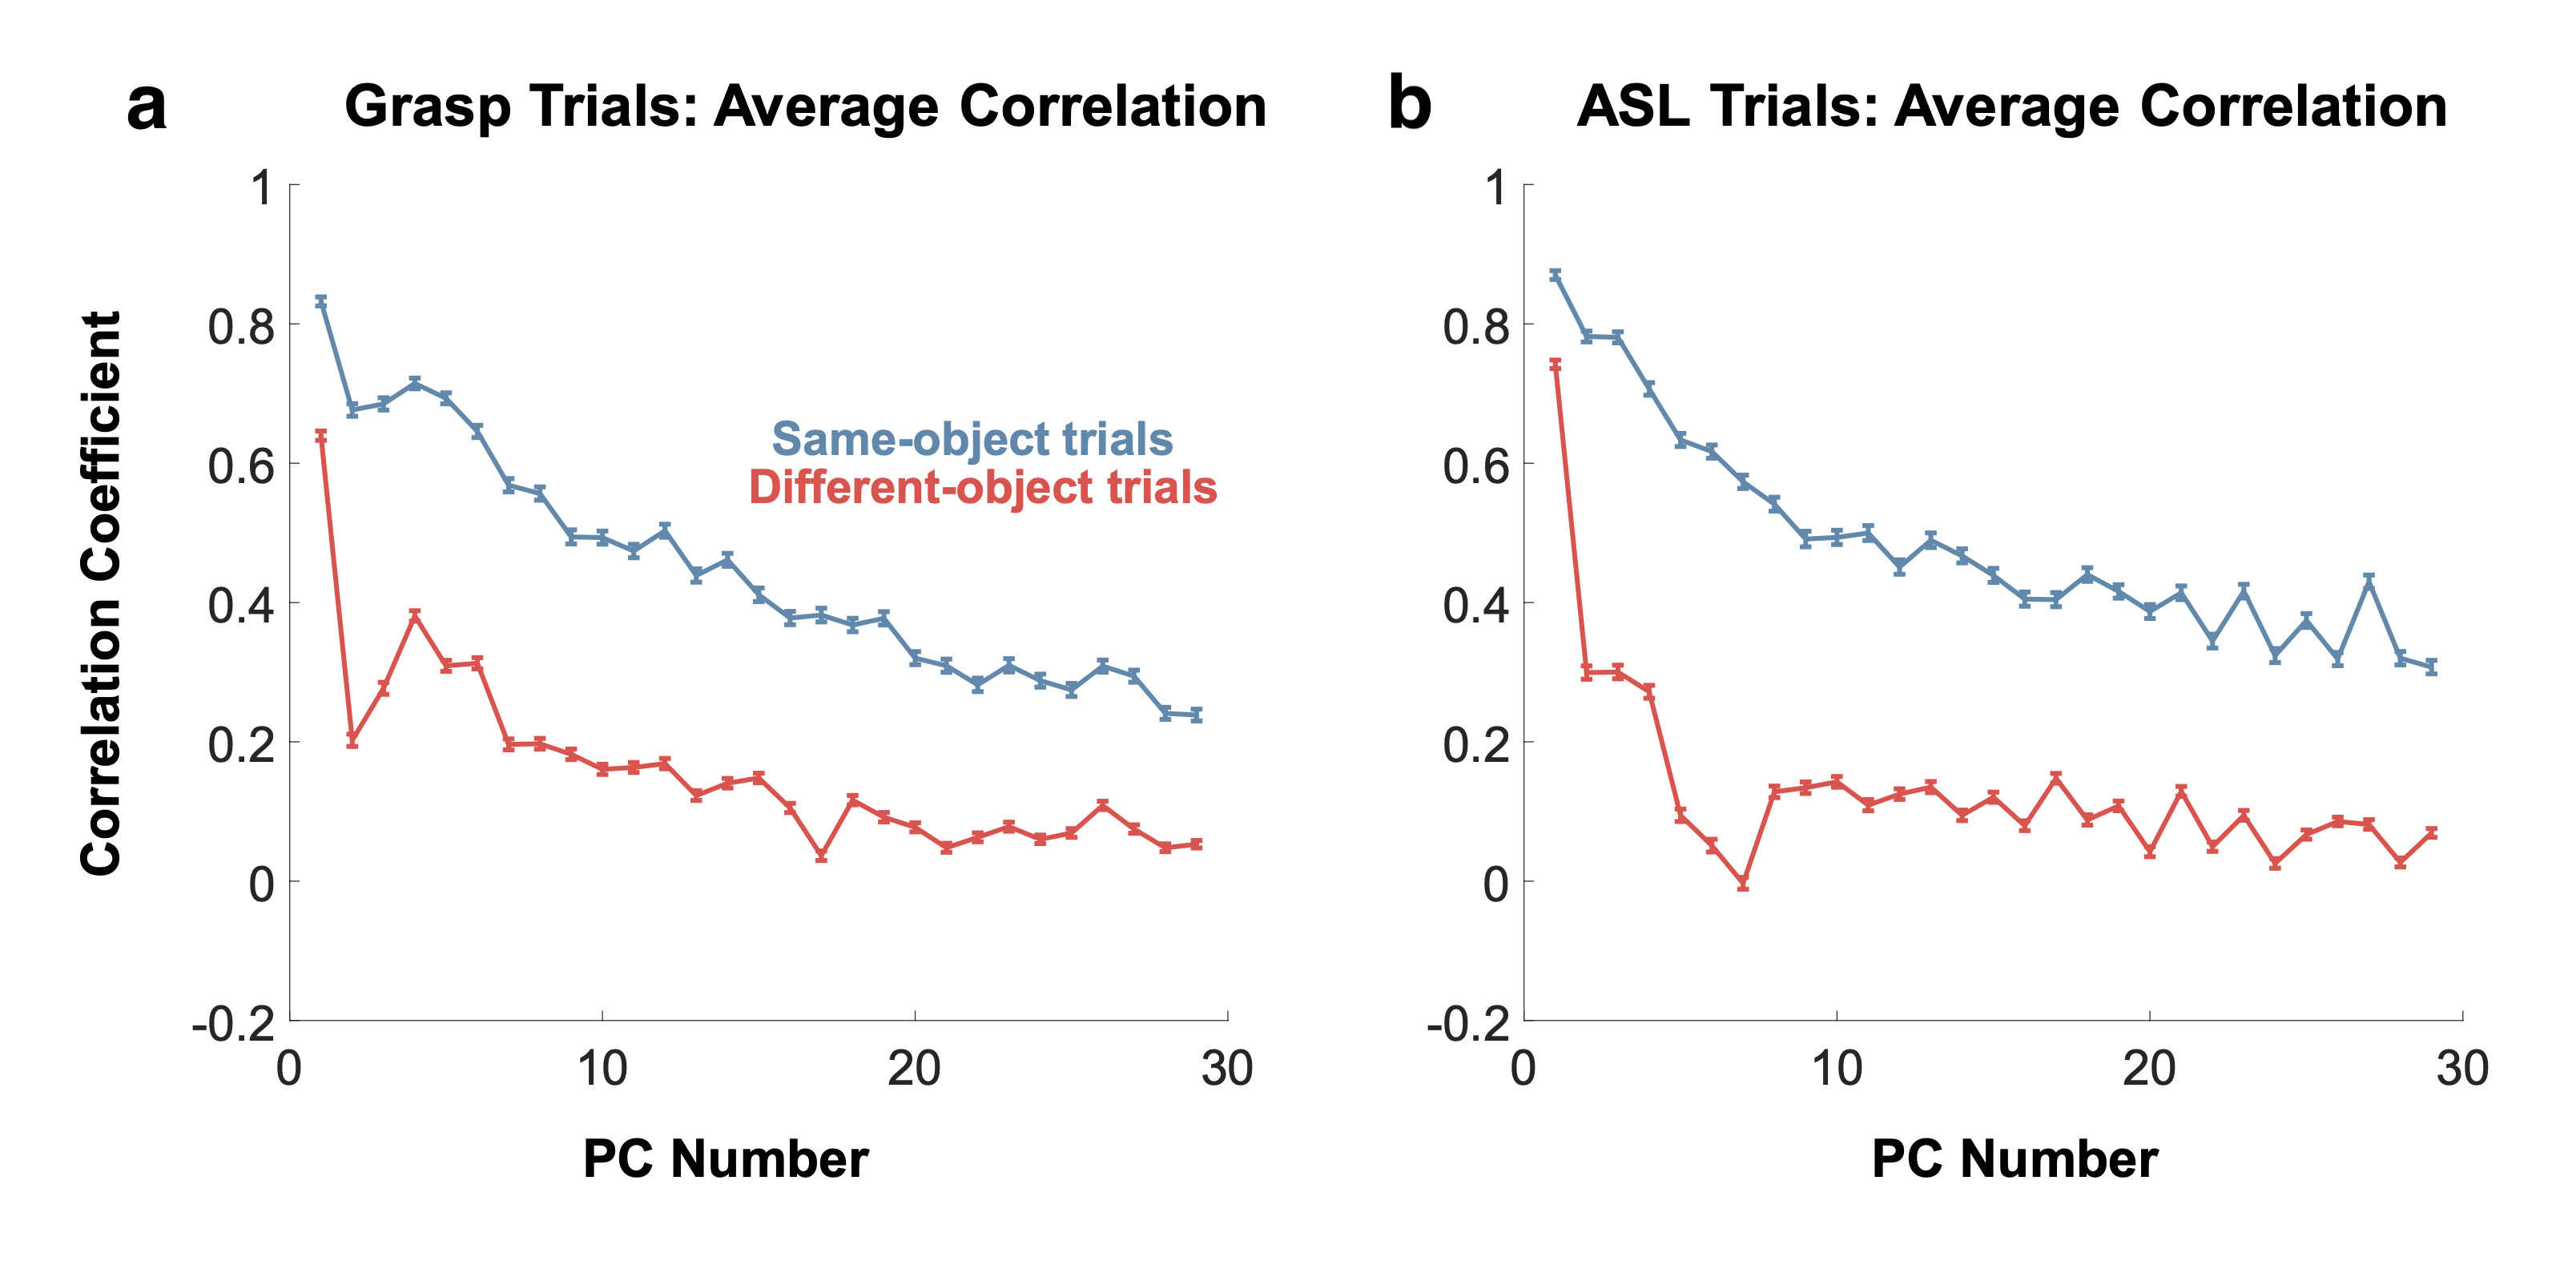
\includegraphics[width=1\textwidth,height=\textheight]{../images/physiology/background/low_variance_PCs.png}
\caption{Taken from Yan et al.~2020. Plots show mean correlations
between hand joint kinematic trajectories during grasp trials with the
same (blue) and different (red) objects (a) and ASL signs (b) projected
onto the same principle components. Correlations are averaged across 8
subjects. Within-object and within-sign correlations are systematically
higher than their shuffled counterparts. Error bars denote SEM. This
data supports the idea that low-variance components of kinematics data
contain task-specific structure rather than merely reflecting noise.
This is encouraging for our experiments, which hope to extend this idea
into careful analyses of task specific features of EMG data across
learning and in response to perturbations.}\label{fig:low_variance_PCs}
\end{figure}

\subsection{Coordinative Structures}\label{coordinative-structures}

Many studies have contributed to the concept of synergies as a
hard-wired organizing feature of the motor
system{[}@mussa-ivaldiMotorLearningCombination2000,@DAvella2003{]}.
However, these works tend to extrapolate from non-primate preparations,
particularly in the frog, and use tasks which are inherently
low-dimensional to explain covariance structure in primate and human
kinematic and electromyography
data{[}@giszterMotorPrimitivesNew2015;@gao2017{]}. That said, it would
be foolish to deny the existence of synergistic muscle coactivation even
at the structural level. Careful studies of force control by the
fingertips present a complex story of dimensionality of control in this
regime{[}@raczSpatiotemporalAnalysisReveals2013{]}. Constraints exist in
the architecture of the hand as well as its control system, though we
maintain that concept of synergies, especially in the context of
dexterous movement, is often presented as an oversimplification rather
than a mere simplification. We believe the story of the hand is more
complex.

Studies have attempted to quantify the number of effective degrees of
freedom of the hand with various methods. This has primarily been taken
to be the number of linear features which contain a desired level of the
original signal variance, where the signal is the joint angles of the
hand engaged in various
behaviors{[}@Ingram2009;@TodorovDimensionality2005{]}. These methods
have resulted in roughly 8 linear features of hand kinematics to solve a
variety of tasks, with subtleties found in inter-task and inter-subject
variations. Note that the motor repertoire is hardly high-dimensional
when compared to the dimensionality of the visual feature extraction
system{[}@yanUnexpectedComplexityEveryday2020{]}. A recent study found
that low-variance linear, kinematic components displayed significantly
higher correlation within condition (e.g.~grasp of a specific object)
than across condition. This suggests that these components carry
task-dependent information rather than condition-independent,
task-irrelevant noise{[}@yanUnexpectedComplexityEveryday2020{]}. This
suggests that the control of the hand is more nuanced than a set of
fixed synergies.

What Bizzi and colleagues call ``the problem of supraspinal pattern
formation''--how synergies are activated through time-- we argue, in the
context of hand control, is not simplified by the existence of
hard-wired or soft-wired
synergies{[}@bizziMotorPlanningExecution2020{]}. Rather, the CNS
produces control signals in a range of contexts and in response to
continually changing task demands. Rather than the CNS ``simplifying
movement'' through synergetic action, it is more likely that hand
synergies fall out of a optimization strategy which trades off effort
and accuracy where effort may, in part, correspond to independent
control of individual control dimensions. In this view, synergies,
hard-wired or not, reflect the statistics of the environment in which
movement is
constructed{[}@brutonSynergiesCoordinationComprehensive2018{]}. If we
limit ourselves to synergetic control, then we have simply passed the
problem to a lower-dimensional one of the same fundamental nature.
Neural control of the hand likely contains a spectrum of modularity in
order to maintain its role as a flexible instrument. Synergetic action
is one end of this spectrum resulting from the computations inherent to,
along with the structures of the human movement machine.

\subsection{Fractionating Structures}\label{fractionating-structures}

Just as many muscle fibers may be innervated by a single AMN, up to
thousands of neurons contact single AMNs through monosynaptic
corticospinal, or corticomotoneuronal (CM), connections and other
descending pathways through elaborate spinal circuitry. The hallmark of
CM connections in particular is their influence over multiple muscle
compartments as well as multiple muscles, though typically agonist or
antagonist sets{[}@cheneyFunctionalClassesPrimate1980{]}. This may seem
counter-intuitive as a means to produce individuated movement, but
experimental evidence in primates has shown that the convergence of many
CM collateral fibers onto single AMNs driving the distal muscles in
particular can produce a fine grading of activity over motor units
driving the distal joints. CM cells also appear to play a role in the
inhibition of antagonist muscles prior to contractions required for
movement {[}@griffinMotorCortexUses2020{]}. These findings confirm
theories about the excitatory and inhibitory role of these connections
dating back decades, and combine to suggest that variables encoded in
cortical ensembles are more complex than kinematics or dynamics
alone{[}@cheneyFunctionalClassesPrimate1980{]}.

The CM tract thus acts in coordination with synergistic muscle
activations of the hand to achieve control that is balanced between
modularity and flexibility. Findings suggest that there is a bipartite
structure in human motor cortex driving dexterous control of the distal
part of the upper limb which, it has been suggested, evolved under
pressure to quickly generalize between tasks. This work argues that
these two streams of hand control, namely ``fractionated'' and
``synergistic'' control, may interact to produce versatility, and
balancing these subsystems may be a key part of the optimization
function when learning new
skills{[}@Rathelot2009;@griffinCorticomotoneuronalCellsAre2015;@Takei2017{]}.
This dualism is likely not rigidly dichotomous, but rather a spectrum of
overriding fractionation (so-called ``New M1'') atop a phylogenetically
older system of synergistic
action{[}@dumCorticospinalSystemStructural2011{]}. Griffin and
colleagues found that CM cells are functionally tuned to a muscle's mode
of activity (agonist, antagonist, fixator) to ``bypass spinal cord
mechanisms and sculpt novel patterns of motor output that are essential
for highly skilled
movements''{[}@griffinCorticomotoneuronalCellsAre2015{]}. The hypothesis
stemming from the previously described work is that CM connections
override the ``consolidated'' patterns putatively generated via spinal
interneuron circuitry. The setup devised in our work aims to measure
fractionation by tracing motor unit correlations across learning.
Whether fractionation in our experiments is due to the CM pathway can
only be speculation, but our work may provide direction for future
studies pairing intracortical recordings with careful electromyography.

\subsection{Supraspinal Motor Maps}\label{supraspinal-motor-maps}

It is known from recent work that primary motor cortex (M1) is not an
isolated movement-generating dynamical system, but rather a node in the
network of a feedback-modulated, distributed movement
machine{[}@sauerbreiCorticalPatternGeneration2019{]}. Thinking of the
structural architecture of M1 as an input-driven system with outputs
along a spectrum of modularity from synergistic to fractionated, we can
ask what kind of functional architecture might have evolved in the
neuromuscular controller? Graziano and colleagues found that 500ms
electrical stimulation to M1 reliably produced stereotyped movements in
primates{[}@graziano2006{]}. These movements appeared to produce
goal-oriented actions pulled out of other contexts such as bringing food
to the mouth, and seemed to be arranged on the cortical sheet
topographically in terms of spatial endpoints rather than as a
humunculus. Graziano refers to this as the cortical ``action map'', that
these stimulations tapped into the control mechanisms of the primate's
motor system{[}@grazianoIntelligentMovementMachine2009{]}. These results
has recently been confirmed by optogenetics work in marmosets and
macaques {[}@ebina2019;@watanabeForelimbMovementsEvoked2020{]}.

The motor map concept suggests interpreting activity in M1 as a field of
feedback control microcircuits, integrating and transforming inputs,
both internal and external, to sculpt ongoing
movement{[}@wiltschkoMappingSubSecondStructure2015{]}. This is in
accordance with the idea that there is a structural hierarchy in M1
covering a spectrum of movement modularity. These ideas together form a
picture of the motor system as a structural scaffold upon which
behaviorally relevant feedback mappings from cortex to the spinal cord
are continuously activated and modulated based on information and
estimates about the periphery. In this view, the encoded variables of
interest depend on the goals, context, and perturbations of the intended
movement. \{+@fig:strick\_graziano\} shows Graziano et al.'s stimulation
results, what might be termed a functional view of the cortical motor
system, next Strick er al.'s described above clarifying the structural
view of modularity in this system.

\begin{figure}
\phantomsection\label{fig:strick_graziano}
\centering
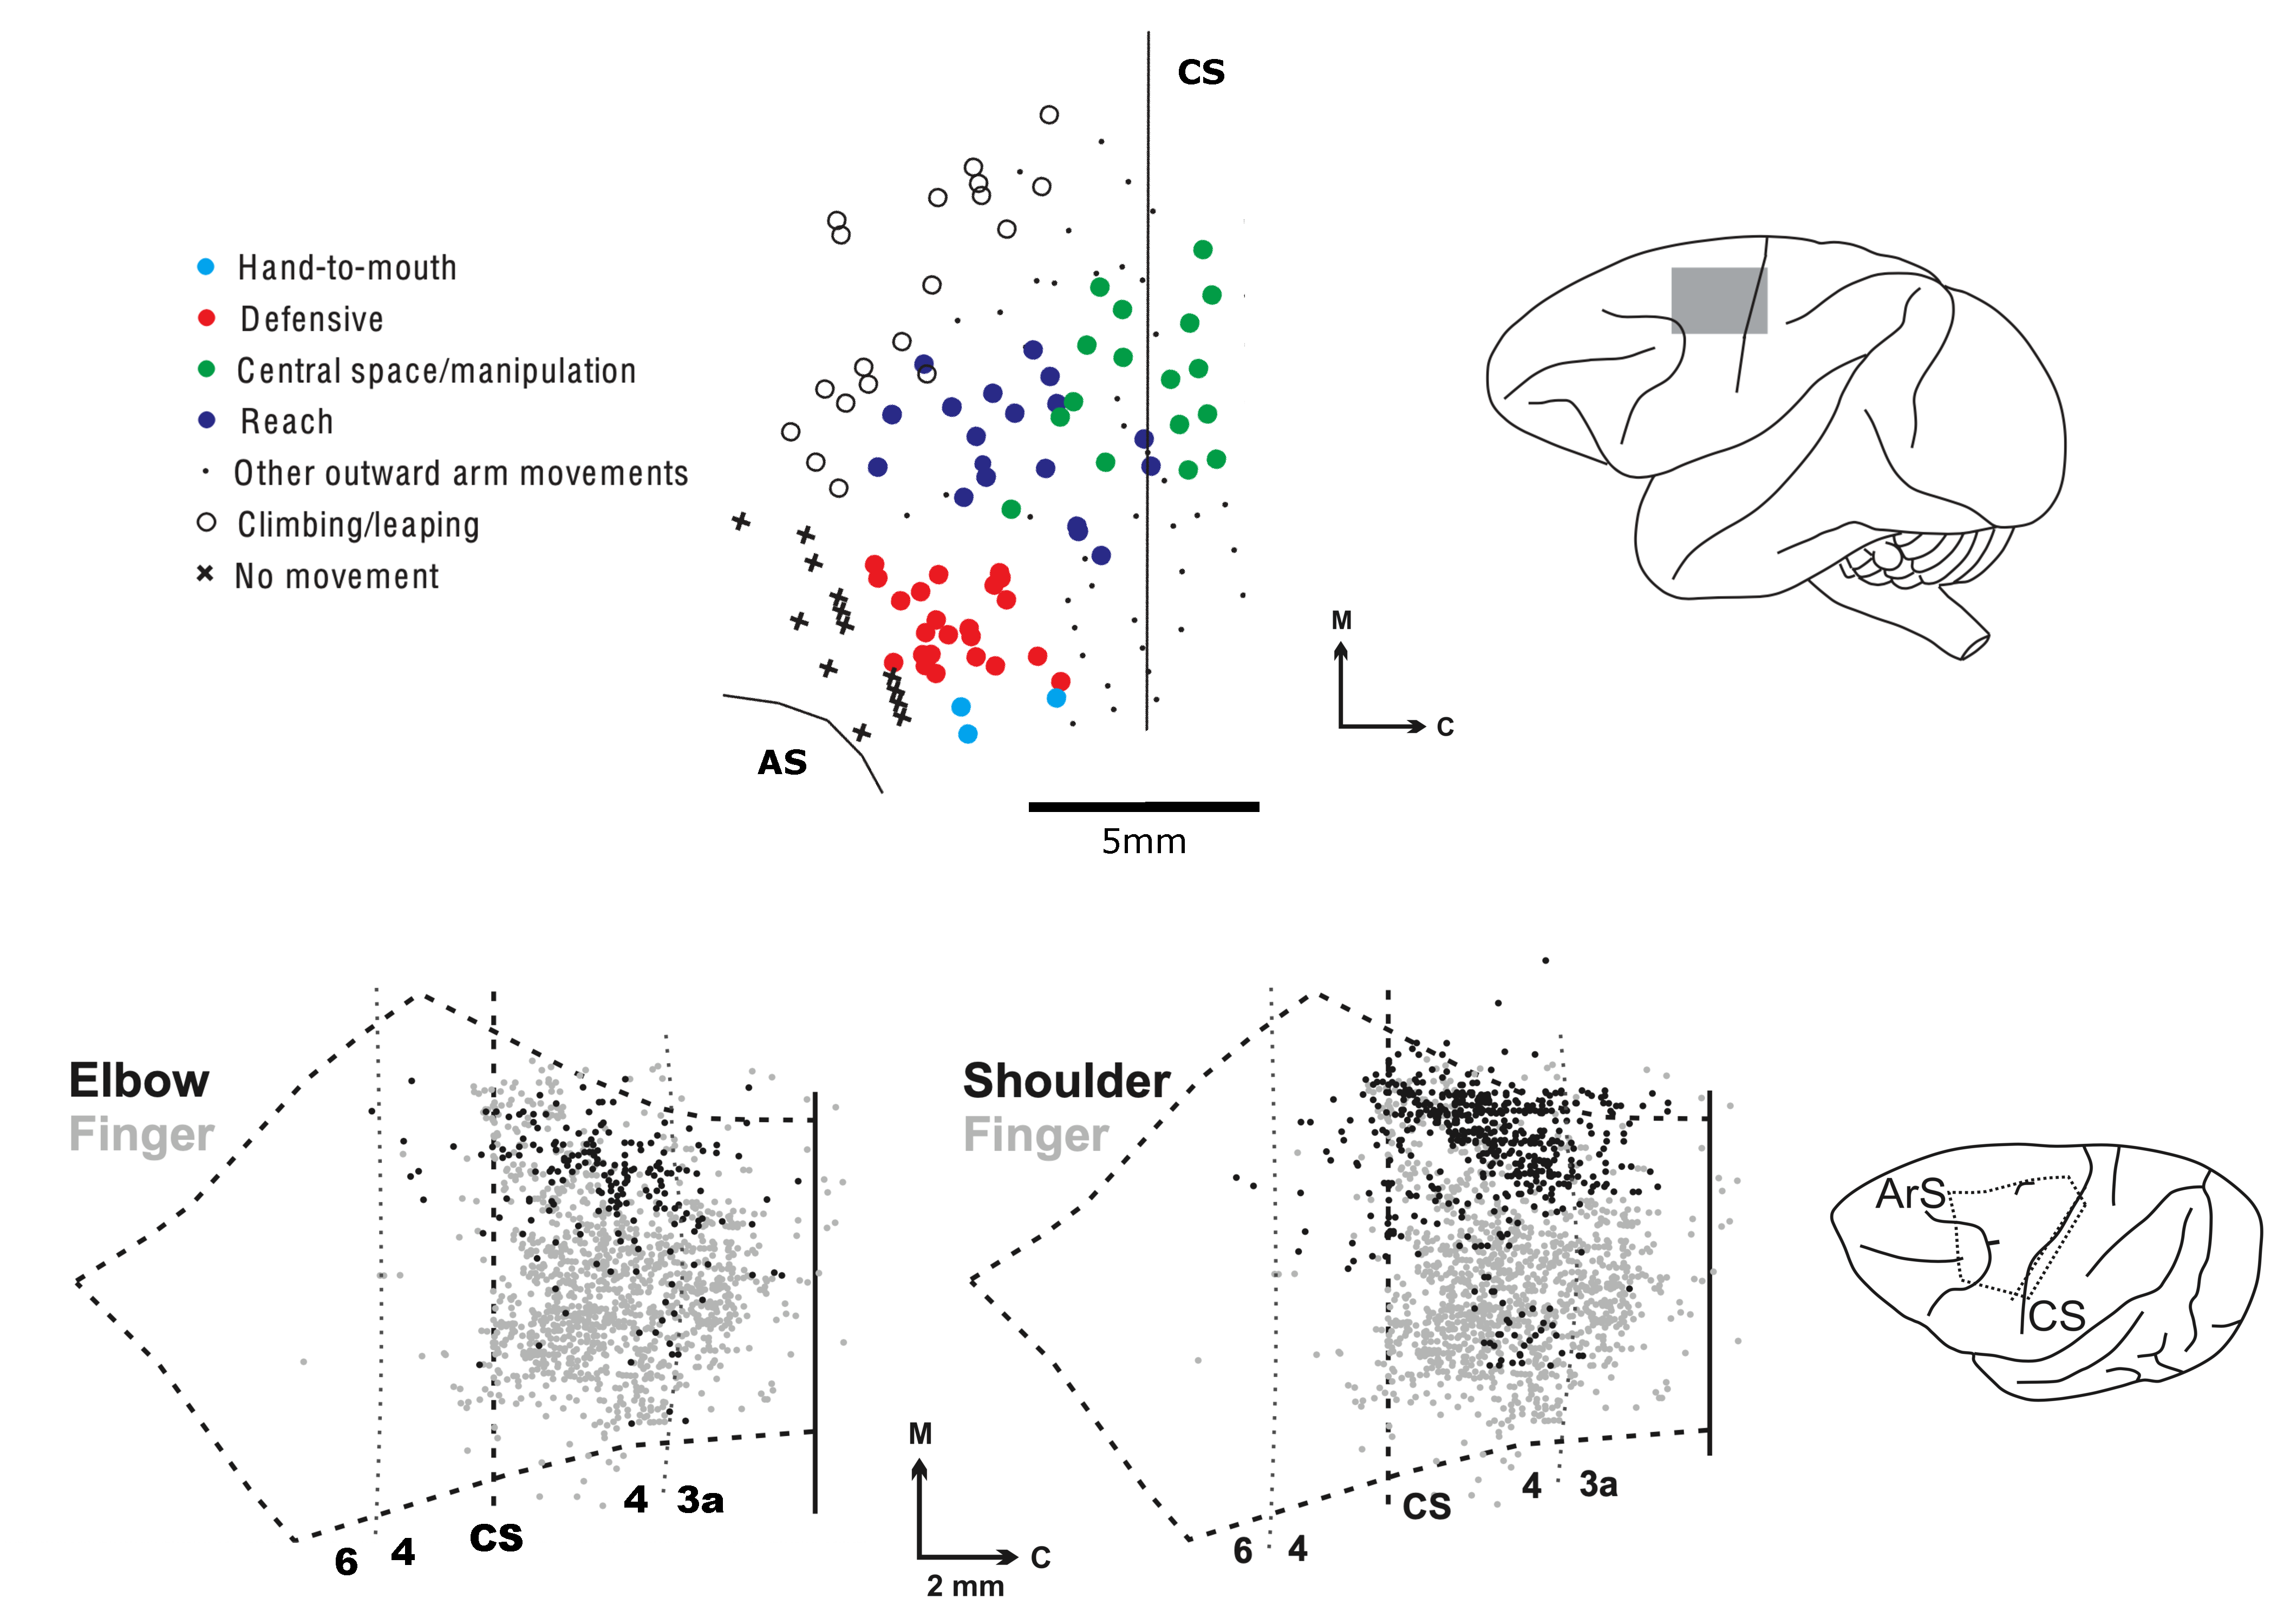
\includegraphics[width=1\textwidth,height=\textheight]{images/physiology/strick_graziano/strick_graziano.pdf}
\caption{Similarities between electrical stimulation on behavorial
timescales and rabies tracing identification of CM cells. CM cells are
largely confined to the caudal half of M1, while this region tends to
evoke complex manipulatory movements when electrically stimulated. (Top
Left) Corticomotoneuronal (CM) cells traced using rabies from muscles of
the elbow and finger. (Top Right) CM cells traced using rabies from
muscles of the shoulder and finger. (Bottom) Complex movements evoked by
500ms electrical stimulation pulse trains. Adapted from Graziano 2005
and Rathelot et
al.~2009{[}@graziano2005;@Rathelot2009{]}.}\label{fig:strick_graziano}
\end{figure}

Graziano writes:

\begin{quote}
``The usefulness of a feedback-dependent mapping from cortex to muscles
is that it can in principle allow neurons in motor cortex to control a
diversity of movement variables, such as direction, speed, hand
position, or posture that transcend a fixed pattern of muscle
activation. If the network receives feedback information about a
specific movement variable, then it can learn to control that
variable.''
\end{quote}

Muscle activity is, in this sense, a readout from a network transforming
state-dependent inputs into movement goals. Rather than choosing muscle
patterns in reconfigurable blocks, it creatively constructs and sculpts
movement. The hierarchy of the motor system may not be rigidly organized
around a particular set of variables. As shown in
\{+@fig:motor\_system\}, many loops exist connecting cortex with the
spinal cord, the cerebellum, the basal ganglia, and the sensorimotor
periphery. Each of these loops contributes information for the flexible
activation of the relevant action maps. Put simply, prevailing evidence
suggests that cerebellar loops provide predictive state information
while basal gangliar loops provide state and/or action value
information. Taken together, this work provides an image of the
incredible complexity which generates dexterous movements of the hand.
This is the foundation on which we can work to build experiments which
elucidate the computations involved in the production of skilled
movement. We aim to connect our results back to what is known about the
system we are attempting to reverse-engineer in order to inspire future
inquiries into the inner workings of the movement machine.

\begin{figure}
\phantomsection\label{fig:motor_system}
\centering
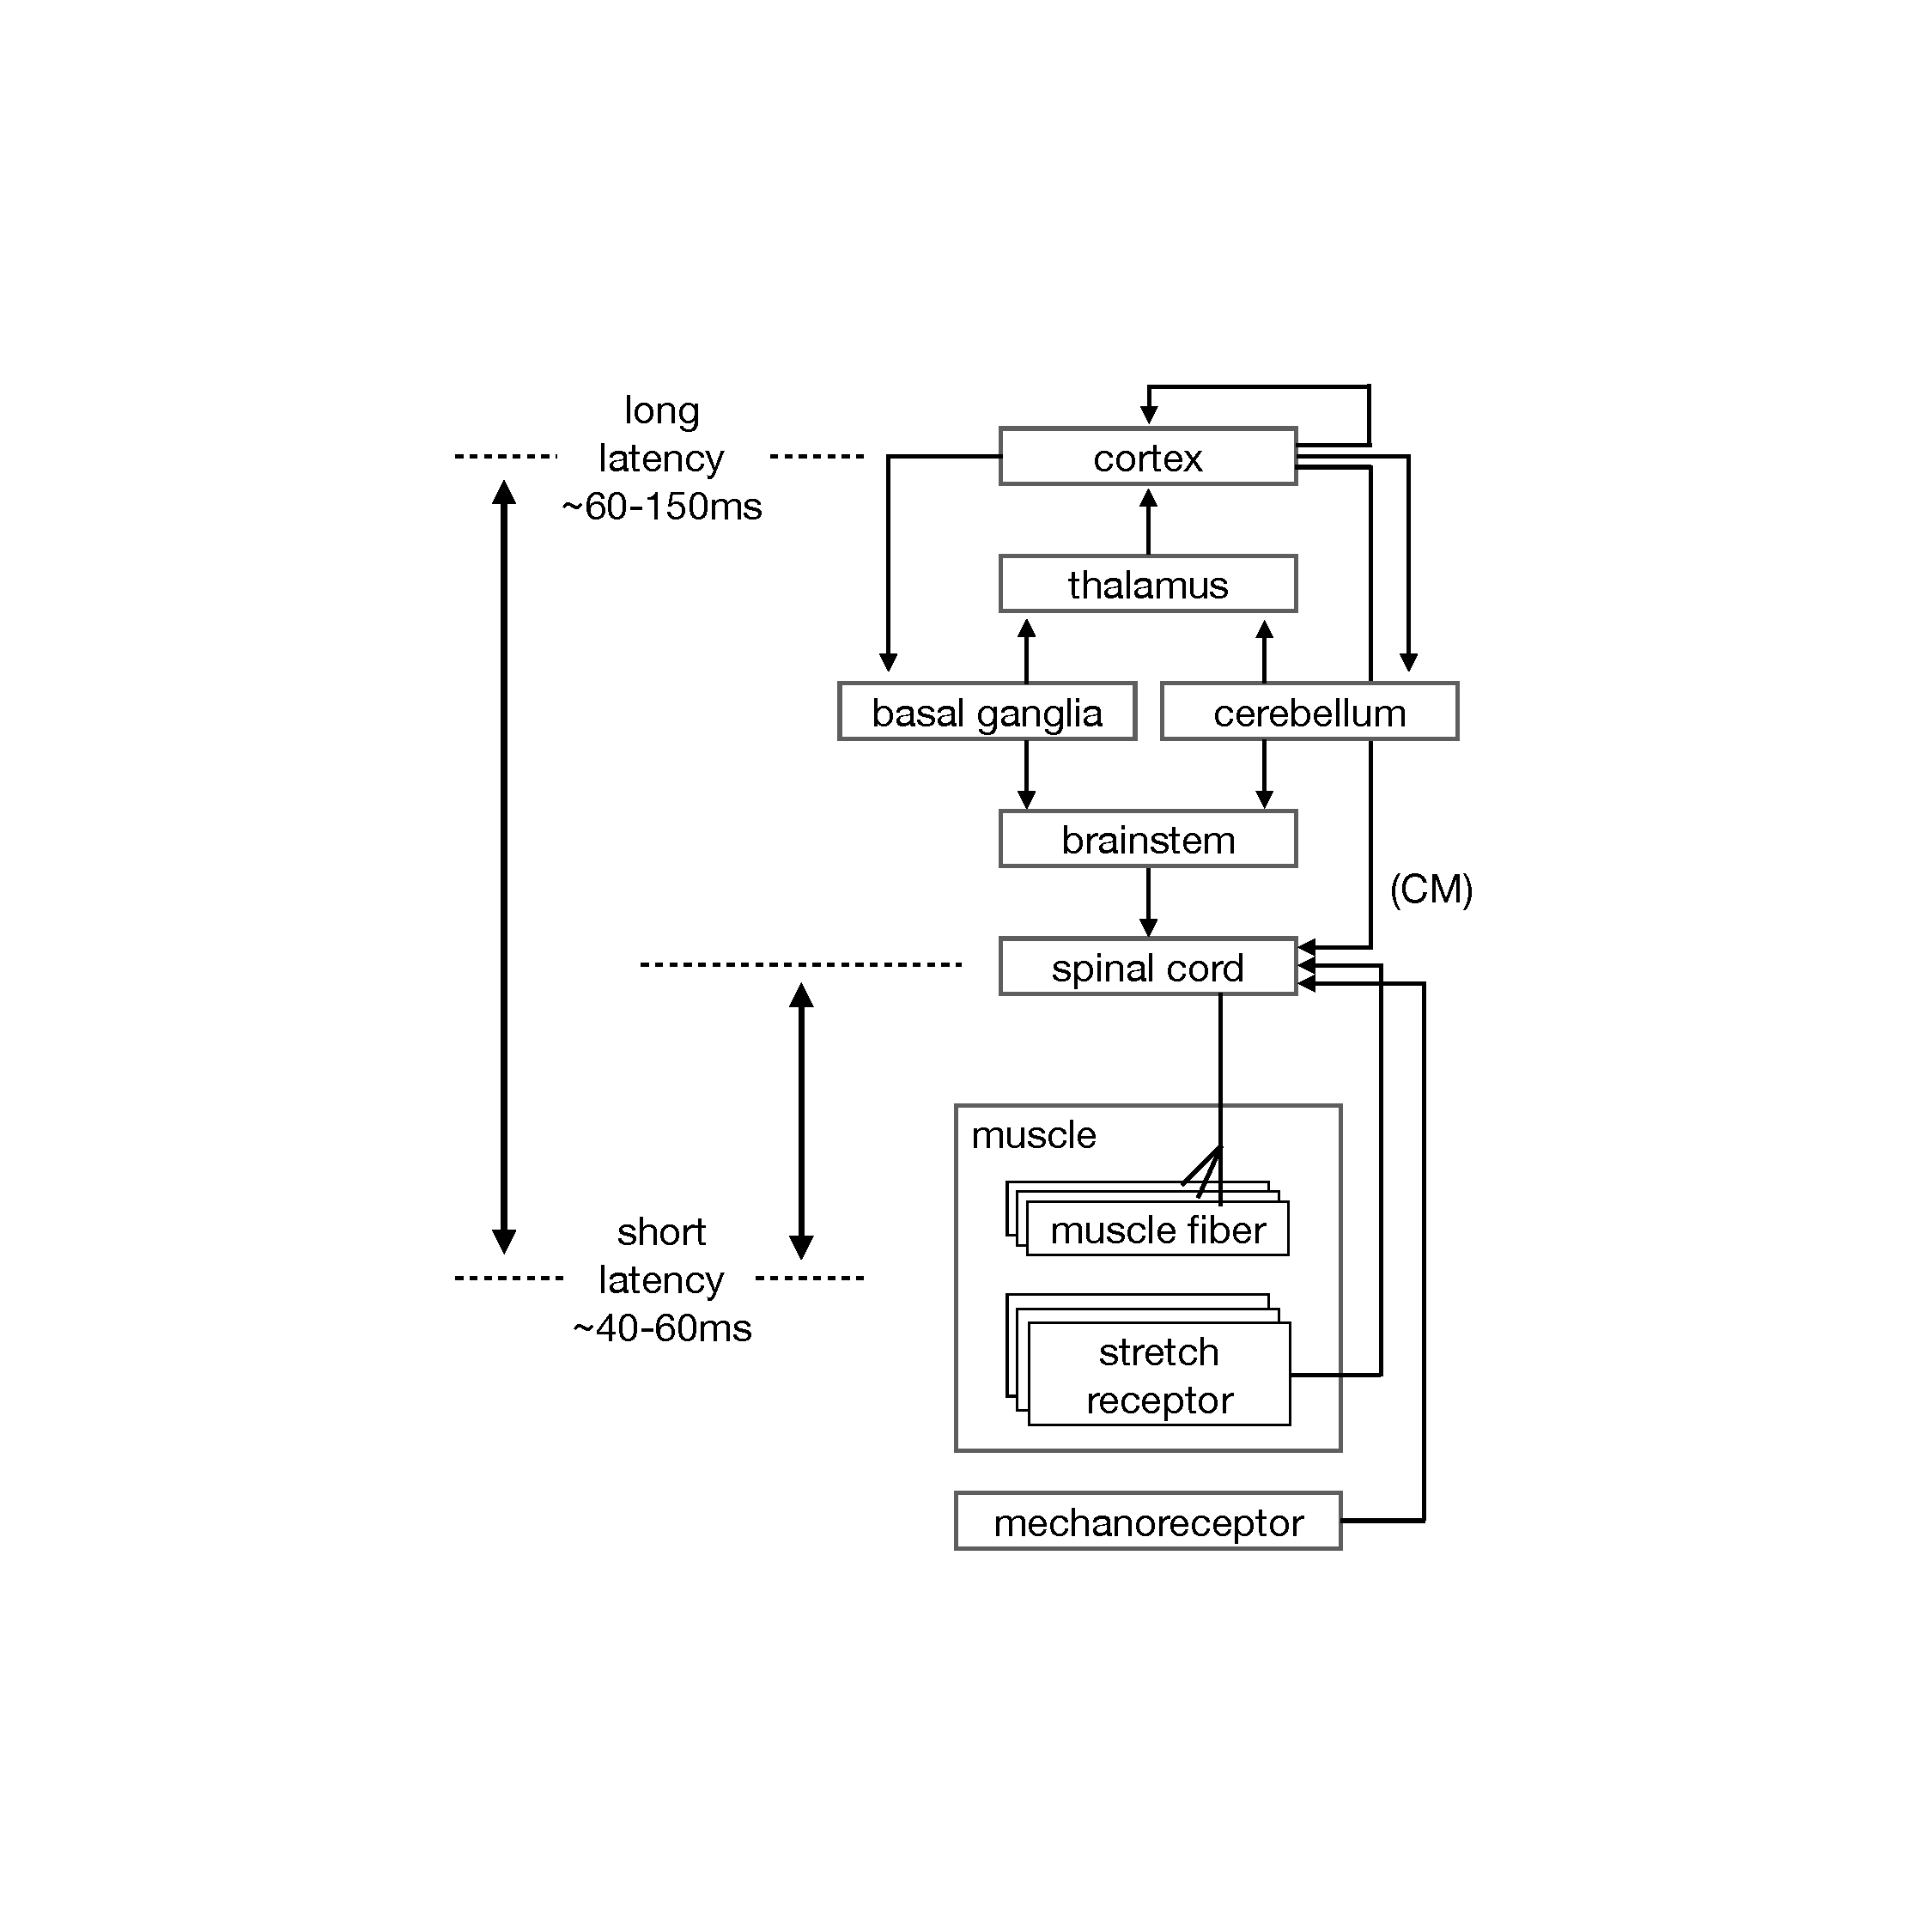
\includegraphics[width=1\textwidth,height=\textheight]{images/physiology/motor_system/motor_system.pdf}
\caption{Overview sketch of the motor system depicting the the
redundancy of the system both hierarchically (multiple muscle fibers are
innervated by the same motor neuron, many motor neurons innervate the
same muscle) as well as heterarchically (parallel spinal,
corticomotoneuronal, cerebellum, basal gangliar feedback loops).
Parallel reflex responses can be classified as long latency
(approximately 60-150ms) and short latency (approximately 60ms). We hope
to consider the parallelism and redundancy of the motor system to
inspire our data analyses and models of motor
computation.}\label{fig:motor_system}
\end{figure}

\subsection{John Rothwell and Jens Bo Nielson: Voluntary
Control}\label{john-rothwell-and-jens-bo-nielson-voluntary-control}

\begin{quote}
In the vast majority of cases, cortical inputs fi rst contact
interneurones which then relay the commands to motoneurones. Since the
same interneurones also receive con -tinuous input from sensory
receptors (and hence might be thought to participate in spinal refl
exes) as well as from interneurones from other parts of the spinal cord,
this means that by the time cortical input reaches motoneurones it has
been fi ltered by multiple lower level systems. In higher primates and
in man, cortical input can access some motoneurones via a special direct
pathway (the corticomotoneuronal pathway), which is often supposed to
play a critical role in volitional movement. However, even if this input
is strong (and there is little comparative evidence on this) the
excitability of motoneurones will have been biased by the multiple other
inputs that each one receives. Thus, even this connection does not
guarantee the brain a straightforward control of muscle.
\end{quote}

\begin{quote}
We argue that distributed cortical projections allow for flexibility of
connections between muscle representations, and therefore are critical
to the flexibility of movements unrestricted by postural demands.
Physiologically, the cortex is the main gateway for visual inputs to
enter and infl uence motor control. This is particularly relevant during
reaching with the arm and during the swing phase of gait for the leg. In
both cases, the limbs are relatively free from feedback control from
gravitational and contact force sensors, and can therefore be driven to
a large extent by visual inputs.
\end{quote}

Posture and contact dictates much of corticospinal function, and we
would expect that these demands influence the architecture of the
underlying circuitry. ``Conscious'' control is likely simply the
availability of visual and propriospinal sensation in the course of the
movement.

\begin{quote}
The anatomy and physiology of the {[}corticospinal{]} connections mean
that if a volitional command were formulated in some hypothetical
centre, it would be extremely diffi cult to predict the consequences
with any certainty unless the state of every interposed connection were
known in advance.
\end{quote}

Nielson argues that hierarchy doesn't function straightforwardly, that
all corticospinal loops can be seen as a collection of distributed,
overlapping modulation of motor neuron activity.

\begin{quote}
About 40 percent of the corticospinal fi bers come from the primary
motor cortex, whereas the cingulate and supplementary areas supply only
about 20 percent each and the premotor areas some 10 percent (Lemon,
2008). All of these areas of cortex also project to brainstem areas that
give rise to reticulospinal tracts, giving them an indirect, cortico-
reticulo-spinal route to the spinal cord as well as the direct
corticospinal route. The primary motor cortex is thought to have fewer
of these indirect connections than other motor areas, suggesting that
its output represents the most `favored' cortical access to spinal cord
circuits.
\end{quote}

\begin{quote}
In primates most of the terminations of the corticospinal tract are on
interneurones in the spinal grey matter with a smaller number of direct
monosynaptic inputs to motoneurones, particularly those inner-vating the
distal muscles of the extremities. These connections represent the only
way the cortex can interact directly with the motor apparatus
(corticomotoneuronal connections).
\end{quote}

\begin{quote}
after pyramidotomy {[}\ldots{]} movements remain slower and fatigued
more rapidly.
\end{quote}

This may be connected to synchronization of the CST? synchronous,
driving input for rapid reactions.

\begin{quote}
We do not know the rules that specify spinal organization in any detail.
However, one striking observation is that most of the connections
between sensory input and motoneurone output are indirect, going via
interneurones rather than direct sensory- motor pathways ( Jankowska,
2001; 2008). An obvious exception to this is the monosynaptic connection
between primary muscle spindle afferents and their homony-mous
motoneurones. However, this seems very much to be a special case rather
than the rule.
\end{quote}

\begin{quote}
One advantage of having interposed interneurones is that they are an
effective way of allowing the spinal circuitry to switch between
different states. For example, in the two funda-mental states of stance
and gait, connectivity during posture should be arranged in order to
resist perturbations of the body whereas during gait postural control
must be released and movement allowed. Going from posture to movement
means turning off the connections that assure stability and turning on
those that allow movement. {[}\ldots{]} A second advantage of
interneurones is that they can specialize in producing different
patterns or rhythms of activity. This could be a special property of
individual neurones or a property of an interconnected network of
neurones, such as envisaged for the locomotor pattern generator.
\end{quote}

Drawing a picture where spinal circuits are autonomous, but modulated,
by cortical input.

\begin{quote}
t is a general fi nding that every single interneu-rone receives input
not only from the sensory modality which is the basis for its classifi
cation (e.g.~as a `Ia inhibitory interneurone', `Ib inhibitory
interneurone', `gr. II interneurone' or `fl exor refl ex afferent
interneurone'), but also from a number of other sensory afferent
modal-ities, other interneurones and a number of descending pathways
(e.g.~corticospinal, vestibu-lospinal, reticulospinal).
\end{quote}

\begin{quote}
It is not an unrealistic possibility that spinal interneurones with a
slight turn of events could have been classifi ed based on their
supraspinal input as taking part in different voluntary movements rather
than the current clas-sifi cation based on afferent input as taking part
in different refl ex actions. This was realized already by Sherrington
(1906) more than 100 years ago when he wrote: ``A simple refl ex is
probably a purely abstract conception, because all parts of the nervous
system are connected together and no part of it is probably ever capable
of reaction without affecting and being affected by various other parts,
and it is a system certainly never absolutely at rest. But the simple
refl ex is a convenient, if not a probable, fi ction.''
\end{quote}

\begin{quote}
\textbf{The discharge of every single motoneurone and thus the
activation of every single muscle fi ber is determined by the integrated
depolarization from on average 10,000 synaptic inputs arising from a
number of different sensory modalities, spinal interneu-rones and
supraspinal control centres.}
\end{quote}

\begin{quote}
Cortical input to the spinal cord should be viewed as using or
modulating the output of the spinal circuitry itself. There is no
separation between `spinal refl exes' and `cortical voluntary movement'.
Instead, it is important to focus on how the neuronal machinery in the
spinal cord may provide an extremely fl exible tool for the execution of
voluntary movements.
\end{quote}

\begin{quote} 
  We hypothesize that there are at least two advantages of cortical control. The fi rst is adaptability which emerges as a consequence of the anatomy of the cortical motor representation. The second is integration of visual input which is particularly important in shaping the hand to manipulate objects. Individuation and precision are secondary consequences of this organization.
\end{quote}

Begs the question of a no-visual experiment?

\begin{quote}
  EMG recordings show that very short synchronous bursts of activity are characteristic of many fractionated fi nger movements, such as writing and tool use {[}\ldots{]} Interposing interneuronal synapses in these connections would tend to remove synchrony and smooth out the command. This is indeed what is seen following corti-cospinal lesion (Farmer et al., 1993). The CM system may thus also be at the heart of human evolution in view of the evolutionary advantage of being able to throw something at an animal in order to kill and eat it.
\end{quote}

\begin{quote} 
  One- third of the cortex, particularly in the parietal and premotor areas, is devoted to visual processing. A considerable part of this is used for shaping/orienting our hand in preparation for grasping and manipulating objects
\end{quote}

\begin{quote} 
  the motor cortex may differ from the spinal cord in degree of fl exibility and a larger possibility of integrating visual input, but otherwise there are no differences between the motor cortex and the spinal cord circuitries (after all CM cells project to motoneurones and receive sensory input much like any good old- fashioned interneurone) that could warrant a signifi cantly different role in our conscious experience of control of the movements that we perform. What we are proposing is that it is not the degree of perceived volition which determines to what extent the motor cortex is involved in a given task, but rather the need for fl exible visual control.
\end{quote}

\begin{quote} 
  We hope that we have made it clear that there is little to support this distinction between automatic and voluntary tasks. We need to consider the integration between supraspinal and spinal control centers for any specifi c task in order to understand how that task is controlled by the nervous system, and try to avoid putting into it volition and voluntary which in any case are terms that belong in philosophy or in specifi c inquiries aimed at unravelling the mechanisms of our cognitive abilities and our conscious experiences.
\end{quote}

Compelling case to look at the entirety of the system, focusing on the contributions that cause motor neurons to fire.

\cleardoublepage\printendnotes%
\ifSubfilesClassLoaded{%
    \newpage%
    \bibliography{../bib/bibliography}%
}{}%
\end{document}